%% 使用 njuthesis 文档类生成南京大学学位论文的示例文档
%%
%% 作者:胡海星,starfish (at) gmail (dot) com
%% 项目主页: http://haixing-hu.github.io/nju-thesis/
%%
%% 本样例文档中用到了吕琦同学的博士论文的提高和部分内容,在此对他表示感谢。
%%
\documentclass[macfonts,master]{njuthesis}
%% njuthesis 文档类的可选参数有:
%%   nobackinfo 取消封二页导师签名信息。注意,按照南大的规定,是需要签名页的。
%%   phd/master/bachelor 选择博士/硕士/学士论文

% 使用 blindtext 宏包自动生成章节文字
% 这仅仅是用于生成样例文档,正式论文中一般用不到该宏包
%\usepackage[math]{blindtext}
\usepackage{listings}
\usepackage{xcolor}

\newcommand\YAMLcolonstyle{\color{red}\mdseries}
\newcommand\YAMLkeystyle{\color{black}\bfseries}
\newcommand\YAMLvaluestyle{\color{blue}\mdseries}

\makeatletter

% here is a macro expanding to the name of the language
% (handy if you decide to change it further down the road)
\newcommand\language@yaml{yaml}

\expandafter\expandafter\expandafter\lstdefinelanguage
\expandafter{\language@yaml}
{
  keywords={true,false,null,y,n},
  keywordstyle=\color{darkgray}\bfseries\small,
  basicstyle=\YAMLkeystyle\small,                                 % assuming a key comes first
  numbers=left,
  numberstyle=\footnotesize,
  frame=single,
  breaklines,
  columns=flexible,
  sensitive=false,
  comment=[l]{\#},
  morecomment=[s]{/*}{*/},
  commentstyle=\color{purple}\ttfamily,
  stringstyle=\YAMLvaluestyle\ttfamily\small,
  moredelim=[l][\color{orange}]{\&},
  moredelim=[l][\color{magenta}]{*},
  moredelim=**[il][\YAMLcolonstyle{:}\YAMLvaluestyle]{:},   % switch to value style at :
  morestring=[b]',
  morestring=[b]",
  literate =    {---}{{\ProcessThreeDashes}}3
                {>}{{\textcolor{red}\textgreater}}1
                {|}{{\textcolor{red}\textbar}}1
                {\ -\ }{{\mdseries\ -\ }}3,
}

% switch to key style at EOL
\lst@AddToHook{EveryLine}{\ifx\lst@language\language@yaml\YAMLkeystyle\fi}
\makeatother

\newcommand\ProcessThreeDashes{\llap{\color{cyan}\mdseries-{-}-}}

%\usepackage[utf8]{inputenc}
%\usepackage[english]{babel}
%
%\usepackage[outputdir=.texpadtmp]{minted}
%\usemintedstyle{borland}

\usepackage{color}
\usepackage{xcolor}

\definecolor{lightgray}{rgb}{.9,.9,.9}
\definecolor{darkgray}{rgb}{.4,.4,.4}
\definecolor{purple}{rgb}{0.65, 0.12, 0.82}

\lstdefinelanguage{Go}{
  % Keywords as defined in the language grammar
  morekeywords=[1]{%
    break,default,func,interface,select,case,defer,go,map,%
    struct,chan,else,goto,package,switch,const,fallthrough,%
    if,range,type, continue,for,import,return,var},
  % Built-in functions
  morekeywords=[2]{%
    append,cap,close,complex,copy,delete,imag,%
    len,make,new,panic,print,println,real,recover},
  % Pre-declared types
  morekeywords=[3]{%
    bool,byte,complex64,complex128,error,float32,float64,%
    int,int8,int16,int32,int64,rune,string,%
    uint,uint8,uint16,uint32,uint64,uintptr},
  % Constants and zero value
  morekeywords=[4]{true,false,iota,nil},
  % Strings : "foo", 'bar', `baz`
  morestring=[b]{"},
  morestring=[b]{'},
  morestring=[b]{`},
  % Comments : /* comment */ and // comment
  comment=[l]{//},
  morecomment=[s]{/*}{*/},
  basicstyle=\ttfamily\small,
  numbers=left,
  numberstyle=\footnotesize,
  frame=single,
  breaklines,
  columns=flexible,
  keywordstyle=\color{blue}\ttfamily,
  stringstyle=\color{red}\ttfamily,
  commentstyle=\color{green}\ttfamily,
  tabsize=4,
  % Options
  sensitive=true
}

\lstdefinelanguage{JavaScript}{
  basicstyle=\ttfamily\small,
  numbers=left,
  numberstyle=\footnotesize,
  frame=single,
  breaklines,
  columns=flexible,
  keywords={typeof, new, true, false, catch, function, return, null, catch, switch, var, if, in, while, do, else, case, break},
  keywordstyle=\color{blue}\bfseries,
  ndkeywords={class, export, boolean, throw, implements, import, this},
  ndkeywordstyle=\color{darkgray}\bfseries,
  identifierstyle=\color{black},
  sensitive=false,
  comment=[l]{//},
  morecomment=[s]{/*}{*/},
  commentstyle=\color{purple}\ttfamily,
  stringstyle=\color{red}\ttfamily,
  morestring=[b]',
  morestring=[b]"
}

\colorlet{punct}{red!60!black}
\definecolor{background}{HTML}{EEEEEE}
\definecolor{delim}{RGB}{20,105,176}
\colorlet{numb}{magenta!60!black}

\lstdefinelanguage{json}{
    basicstyle=\ttfamily\small,
    numbers=left,
    numberstyle=\footnotesize,
    frame=single,
  	breaklines,
  	columns=flexible,
    stepnumber=1,
    numbersep=8pt,
    showstringspaces=false,
    breaklines=true,
    frame=lines,
    backgroundcolor=\color{background},
    literate=
     *{0}{{{\color{numb}0}}}{1}
      {1}{{{\color{numb}1}}}{1}
      {2}{{{\color{numb}2}}}{1}
      {3}{{{\color{numb}3}}}{1}
      {4}{{{\color{numb}4}}}{1}
      {5}{{{\color{numb}5}}}{1}
      {6}{{{\color{numb}6}}}{1}
      {7}{{{\color{numb}7}}}{1}
      {8}{{{\color{numb}8}}}{1}
      {9}{{{\color{numb}9}}}{1}
      {:}{{{\color{punct}{:}}}}{1}
      {,}{{{\color{punct}{,}}}}{1}
      {\{}{{{\color{delim}{\{}}}}{1}
      {\}}{{{\color{delim}{\}}}}}{1}
      {[}{{{\color{delim}{[}}}}{1}
      {]}{{{\color{delim}{]}}}}{1},
}

%%%%%%%%%%%%%%%%%%%%%%%%%%%%%%%%%%%%%%%%%%%%%%%%%%%%%%%%%%%%%%%%%%%%%%%%%%%%%%%
% 设置《国家图书馆封面》的内容,仅博士论文才需要填写

% 设置论文按照《中国图书资料分类法》的分类编号
\classification{0175.2}
% 论文的密级。需按照GB/T 7156-2003标准进行设置。预定义的值包括:
% - \openlevel,表示公开级:此级别的文献可在国内外发行和交换。
% - \controllevel,表示限制级:此级别的文献内容不涉及国家秘密,但在一定时间内
%   限制其交流和使用范围。
% - \confidentiallevel,表示秘密级:此级别的文献内容涉及一般国家秘密。
% - \clasifiedlevel,表示机密级:此级别的文献内容涉及重要的国家秘密 。
% - \mostconfidentiallevel,表示绝密级:此级别的文献内容涉及最重要的国家秘密。
% 此属性可选,默认为\openlevel,即公开级。
\securitylevel{\controllevel}
% 设置论文按照《国际十进分类法UDC》的分类编号
% 该编号可在下述网址查询:http://www.udcc.org/udcsummary/php/index.php?lang=chi
\udc{004.72}
% 国家图书馆封面上的论文标题第一行,不可换行。此属性可选,默认值为通过\title设置的标题。
\nlctitlea{声明式的通用Kubernetes}
% 国家图书馆封面上的论文标题第二行,不可换行。此属性可选,默认值为空白。
\nlctitleb{Operator的设计与实现}
% 国家图书馆封面上的论文标题第三行,不可换行。此属性可选,默认值为空白。
\nlctitlec{}
% 导师的单位名称及地址
\supervisorinfo{南京大学计算机科学与技术系~~南京市栖霞区仙林大道163号~~210023}
% 答辩委员会主席
\chairman{~~教授}
% 第一位评阅人
\reviewera{~~教授}
% 第二位评阅人
\reviewerb{~~副教授}
% 第三位评阅人
\reviewerc{~~教授}
% 第四位评阅人
\reviewerd{~~研究员}

%%%%%%%%%%%%%%%%%%%%%%%%%%%%%%%%%%%%%%%%%%%%%%%%%%%%%%%%%%%%%%%%%%%%%%%%%%%%%%%
% 设置论文的中文封面

% 论文标题,不可换行
\title{声明式的通用Kubernetes Operator的设计与实现}
\titlea{声明式的通用Kubernetes}
\titleb{Operator的设计与实现}
% 如果论文标题过长,可以分两行,第一行用\titlea{}定义,第二行用\titleb{}定义,将上面的\title{}注释掉
% \titlea{半轻衰变$D^+\to \omega(\phi)e^+\nu_e$的研究}
% \titleb{和弱衰变$J/\psi \to D_s^{(*)-}e^+\nu_e$的寻找}

%%盲审命令,空白字段设置请看.cls文件\newcommand*{\blind}
%此外,请按照盲审要求自行去掉个人简历、致谢等页面中的个人信息
%\blind

% 论文作者姓名
\author{汪浩港}
% 论文作者联系电话
\telphone{15605213809}
% 论文作者电子邮件地址
\email{whg19961229@gmail.com}
% 论文作者学生证号
\studentnum{MG1833067}
% 论文作者入学年份(年级)
\grade{2018}
% 导师姓名职称
\supervisor{曹春~~教授}
% 导师的联系电话
\supervisortelphone{18951679203}
% 论文作者的学科与专业方向
\major{计算机科学与技术}
% 论文作者的研究方向
\researchfield{软件方法学}

% 论文作者所在院系的中文名称
\department{计算机科学与技术系}
% 论文作者所在学校或机构的名称。此属性可选,默认值为``南京大学''。
\institute{南京大学}
% 论文的提交日期,需设置年、月、日。
\submitdate{2021年4月15日}
% 论文的答辩日期,需设置年、月、日。
\defenddate{2021年6月1日}
% 论文的定稿日期,需设置年、月、日。此属性可选,默认值为最后一次编译时的日期,精确到日。
%% \date{2013年5月1日}
% 论文的定稿日期,需设置年、月、日。此属性可选,默认值为最后一次编译时的日期,精确到日。
%% \date{2013年5月1日}

%%%%%%%%%%%%%%%%%%%%%%%%%%%%%%%%%%%%%%%%%%%%%%%%%%%%%%%%%%%%%%%%%%%%%%%%%%%%%%%
% 设置论文的英文封面

% 论文的英文标题,不可换行
\englishtitle{The Design and Implementation of A Declarative Universal Kubernetes Operator}
% 论文作者姓名的拼音
\englishauthor{Wang Haogang}
% 导师姓名职称的英文
\englishsupervisor{Professor Cao Chun}
% 论文作者学科与专业的英文名
\englishmajor{Computer Science and Technology}
% 论文作者所在院系的英文名称
\englishdepartment{Department of Computer Science and Technology}
% 论文作者所在学校或机构的英文名称。此属性可选,默认值为``Nanjing University''。
\englishinstitute{Nanjing University}
% 论文完成日期的英文形式,它将出现在英文封面下方。需设置年、月、日。日期格式使用美国的日期
% 格式,即``Month day, year'',其中``Month''为月份的英文名全称,首字母大写;``day''为
% 该月中日期的阿拉伯数字表示;``year''为年份的四位阿拉伯数字表示。此属性可选,默认值为最后
% 一次编译时的日期。
\englishdate{Apr 15, 2021}

%%%%%%%%%%%%%%%%%%%%%%%%%%%%%%%%%%%%%%%%%%%%%%%%%%%%%%%%%%%%%%%%%%%%%%%%%%%%%%%
% 设置论文的中文摘要

% 设置中文摘要页面的论文标题及副标题的第一行。
% 此属性可选,其默认值为使用|\title|命令所设置的论文标题
% \abstracttitlea{数据中心网络模型研究}
% 设置中文摘要页面的论文标题及副标题的第二行。
% 此属性可选,其默认值为空白
% \abstracttitleb{}

%%%%%%%%%%%%%%%%%%%%%%%%%%%%%%%%%%%%%%%%%%%%%%%%%%%%%%%%%%%%%%%%%%%%%%%%%%%%%%%
% 设置论文的英文摘要

% 设置英文摘要页面的论文标题及副标题的第一行。
% 此属性可选,其默认值为使用|\englishtitle|命令所设置的论文标题
\englishabstracttitlea{The Design and Implementation of A Declarative}
% 设置英文摘要页面的论文标题及副标题的第二行。
% 此属性可选,其默认值为空白
\englishabstracttitleb{Universal Kubernetes Operator}

%%%%%%%%%%%%%%%%%%%%%%%%%%%%%%%%%%%%%%%%%%%%%%%%%%%%%%%%%%%%%%%%%%%%%%%%%%%%%%%
\begin{document}

%%%%%%%%%%%%%%%%%%%%%%%%%%%%%%%%%%%%%%%%%%%%%%%%%%%%%%%%%%%%%%%%%%%%%%%%%%%%%%%

% 制作国家图书馆封面(博士学位论文才需要)
%\makenlctitle
% 制作中文封面
\maketitle
% 制作英文封面
\makeenglishtitle


%%%%%%%%%%%%%%%%%%%%%%%%%%%%%%%%%%%%%%%%%%%%%%%%%%%%%%%%%%%%%%%%%%%%%%%%%%%%%%%
% 开始前言部分
\frontmatter

%%%%%%%%%%%%%%%%%%%%%%%%%%%%%%%%%%%%%%%%%%%%%%%%%%%%%%%%%%%%%%%%%%%%%%%%%%%%%%%
% 论文的中文摘要
\begin{abstract}
Kubernetes是最受欢迎的容器编排系统,它可以实现应用的自动化部署,已经成为分布式资源调度和自动化运维的事实标准。为了适应成千上万的应用的工作模式,Kubernetes Operators被官方推荐作为在Kubernetes中打包、部署和管理应用的方法,它是用户扩展Kubernetes的声明式API的最主流的方式。本文工作针对Kubernetes Operator开发中存在的学习曲线陡峭、非功能性代码繁多、模版代码冗余等问题,研究了Operator的工作原理,提出了一种声明式的通用Kubernetes Operator,将其命名为UniversalController,简称UC,从而更简单地开发和部署自定义控制器。具体而言,本文工作的主要内容包括:
\begin{enumerate}
	\item 针对Operator开发困难的问题,提出一种声明式的通用调谐技术,简化需要编写的代码,大量减少Operator开发者的工作量,免除学习Kubernetes客户端库、Kubernetes API机制库或其他工具的负担,也不用去编写或生成模版代码,而是将精力集中在业务逻辑上,即描述期望状态上。
	\item 实现了声明式的通用Kubernetes Operator,UC。该工具具有声明式的资源监视(watch),声明式的调谐、声明式的更新策略和语言无关的特性。用户不需要编写任何与Kubernetes交互的代码,只需要在YAML文件中描述需要监听的资源、使用的更新策略以及在调谐代码段中描述期望的状态即可。
	\item 基于UC重新实现了一些现有的Operator,证明了UniversalController可以极大的缩减开发工作量,并且适用于大部分场景的开发。同时性能测试验证了它还能在多自定义控制器部署的环境中减少内存消耗和kube-apiserver的负载。
\end{enumerate}

% 中文关键词。关键词之间用中文全角分号隔开,末尾无标点符号。
\keywords{Kubernetes;Operator;声明式;UniversalController}
\end{abstract}

%%%%%%%%%%%%%%%%%%%%%%%%%%%%%%%%%%%%%%%%%%%%%%%%%%%%%%%%%%%%%%%%%%%%%%%%%%%%%%%
% 论文的英文摘要
\begin{englishabstract}
% 英文关键词。关键词之间用英文半角逗号隔开,末尾无符号。
Kubernetes is the most popular container orchestration system for automating application deployment and has become the fact standard for distributed resource scheduling and automated operations and maintenance. To accommodate the working patterns of thousands of applications, Kubernetes Operators are officially recommended as the way to package, deploy and manage applications in Kubernetes, and it is the most mainstream way for users to scale Kubernetes. The work in this paper addresses the problems of Kubernetes Operator development, such as steep learning curve, extensive non-functional code, and redundant template code. This paper investigates how Operators work, and proposes a declarative universal Kubernetes Operator, which is named UniversalController, or UC for short. UniversalController is helpful for developing and deploying custom controllers.Specifically, the main elements of the work in this paper include:

\begin{enumerate}
	\item To address the problem of difficult Operator development, a declarative universal reconciliation technique is proposed to simplify the code that needs to be written, to massively reduce the workload of Operator developers, to eliminate the burden of learning the Kubernetes client library, the Kubernetes API mechanism library or other tools, and to not have to write or generate template code, but to focus on business logic, i.e., describing the desired state.
	\item Implements a declarative universal Kubernetes Operator, named as UniversalController, with declarative resource watch, declarative reconciliation, declarative update policies, and language-agnostic features. Instead of writing any code to interact with Kubernetes, users only need to describe the resources to be listened to, the update policies to be used in a YAML file and the desired state in the reconciliation snippet.
	\item Based on UniversalController, some existing Operators were re-implemented, proving that UniversalController can greatly reduce development effort and is suitable for most scenarios. Performance testing also verified that it can reduce memory consumption and kube-apiserver load in environments with multiple custom controller deployments.
\end{enumerate}

\englishkeywords{Kubernetes;Operator;Declarative;UniversalController}
\end{englishabstract}

%%%%%%%%%%%%%%%%%%%%%%%%%%%%%%%%%%%%%%%%%%%%%%%%%%%%%%%%%%%%%%%%%%%%%%%%%%%%%%%
% 生成论文目次
\tableofcontents

%%%%%%%%%%%%%%%%%%%%%%%%%%%%%%%%%%%%%%%%%%%%%%%%%%%%%%%%%%%%%%%%%%%%%%%%%%%%%%%
% 生成插图清单。如无需插图清单则可注释掉下述语句。
\listoffigures

%%%%%%%%%%%%%%%%%%%%%%%%%%%%%%%%%%%%%%%%%%%%%%%%%%%%%%%%%%%%%%%%%%%%%%%%%%%%%%%
% 生成附表清单。如无需附表清单则可注释掉下述语句。
\listoftables

%%%%%%%%%%%%%%%%%%%%%%%%%%%%%%%%%%%%%%%%%%%%%%%%%%%%%%%%%%%%%%%%%%%%%%%%%%%%%%%
% 开始正文部分
\mainmatter

%%%%%%%%%%%%%%%%%%%%%%%%%%%%%%%%%%%%%%%%%%%%%%%%%%%%%%%%%%%%%%%%%%%%%%%%%%%%%%%
% 学位论文的正文应以《绪论》作为第一章
\chapter{绪论}\label{chapter_introduction}
\section{研究背景}

在过去十年中,软件和IT系统的开发、托管、交付和扩展方式发生了根本性的转变。大规模分布式应用不断产生,新的需求也不断产生,集群管理人员希望应用能够快速适应用户流量的波动,同时最大限度地降低IT基础设施的管理成本,这些都为云技术被广泛采用铺平了道路。正如Netflix或Zalando等颇具规模的互联网科技公司所展示的那样,软件开发的方式和方法已经从每年几次的大型单体应用的计划驱动交付转变为由数百个单一用途的服务组成的系统,每个服务都是独立和可多次部署的,一个服务往往一天内就有多个版本的迭代\cite{zalando}\cite{netflix}。

尽管云计算具有相当的灵活性,但随着应用和平台的复杂性增加,仍然需要对基础应用、基础设施和相关流程进行创新与改进。应用程序和基础设施运营团队在管理基础设施方面正面临着挑战,这些基础设施需要同时支持数百甚至数千的应用程序。在这种情况下,传统的自动化方法,如使用特制的、指令式的脚本,被证明是难以管理和扩展的。相反,最近越来越流行的自动化工具旨在遵循基础设施即代码(Infrastructure as code,IaC)原则。根据这一原则,基础设施和核心服务的整体配置和状态要用(典型的声明性)代码来定义。然后,借助相关工具,这个刻画了期望状态定义的代码,可以自动转换为正确的指令和API调用,从而产生完全符合期望状态的配置资源。这种将期望状态的定义与实际状态同步的过程被称为``状态调谐'',一些现代的基础设施和云计算自动化工具都采用了这种方法,其中最受欢迎的是Terraform和基于容器的平台Kubernetes。

Kubernetes已经开始被广泛应用于基础设施自动化和状态调谐的使用场景。它是目前最受欢迎的管理基于容器的应用程序的平台,它从一开始就围绕着状态调谐的概念设计。整个架构可以被认为是一个各个模块通过共享状态存储协作的调谐循环系统。此外,可扩展性是Kubernetes设计中的一个核心方面。通过结合这两个特点,Kubernetes也被用作一个通用的状态调谐引擎,能够调谐定制的、特定于应用程序的资源和状态,这些资源和状态甚至可以是Kubernetes本身的外部资源,如云提供商资源或虚拟数据中心设备。为了利用这些功能,应用程序需要正确有效地处理与Kubernetes API的通信和集成,这些并不是简单的工作。由于Kubernetes仍然是一个相对年轻的项目,试图解决这种复杂性的可用库非常少。Kubernetes本身与许多其他容器和云原生技术类似,是用Go语言编写的,所以最成熟的集成和扩展库也是用Go语言编写的。也就是说,只要相关的代码都可以用Go语言编写,开发体验会是最好的。这对于一部分开发者和公司是可能的,但大部分其他语言的开发者将不得不放弃许多已有的标准和工具。更先进、支持更多编程语言的Kubernetes抽象库才会让更多人收益。

Kubernetes具有很好的开放性与可拓展性,开发人员可以通过Operator来拓展Kubernetes的声明式API,这也是最常用的方式。Operator的概念是由coreOS提出的,是对Kubernetes的软件拓展,帮助实现应用程序的自动化部署、升级、管理以及运维\cite{operators}。然而,编写一个Operator并不容易,具有相当高的门槛,并且需要付出大量的精力和时间。Operator开发人员需要具备一定程度的Kubernetes和分布式系统知识,需要写大量的模版代码或者使用代码生成工具。编写出的Operator帮助我们实现了应用程序的自动化运维,但是维护这个Operator却还是要给开发人员带来很大的负担\cite{problemofoperators}。因此诞生了很多工具,它们都希望帮助开发人员更简单的实现自己的Operator。本文提出的UniversalController是一个声明式的通用Operator,可以有效减轻开发人员的开发与运维负担。

\section{研究现状}

在开发Operator时,最常用且灵活的做法是使用现有的Kubernetes客户端,可以是Go、Java、JS/Typescript或其他语言的客户端。这些客户端提供了对Kubernetes API的直接底层访问,没有任何包装或附加层。其中最成熟且功能齐全的是Go客户端client-go\footnote{https://github.com/kubernetes/client-go},它提供了很多基础组件用于自动以控制器的开发。但是client-go不是一个专门用于实现控制器的库,而是为了更通用的场景而设计的,用它来实现Operator还是需要接触到太多的底层接口,十分繁琐。而如果用Go以外的编程语言,体验更是会大幅下滑,它们没有client-go成熟,甚至缺少很多特性。

为了简化Kubernetes Operator的开发,目前的方法主要是使用SDK工具,它使用代码生成工具来生成模版代码,帮助用户搭建项目基础脚手架。

Kubernetes-sigs\footnote{https://github.com/kubernetes-sigs}团队开源的kubebuilder和coreOS开源的Operator SDK都是基于这个思路而产生的。与Ruby on Rails和SpringBoot等Web开发框架类似,Kubebuilder和Operator SDK提高了开发人员使用Go语言快速构建和发布Kubernetes API的速度并降低了管理的复杂性。它们都使用了高级抽象库controller-runtime\footnote{https://github.com/kubernetes-sigs/controller-runtime},建立在用于构建核心Kubernetes API的规范技术之上,以提供简单的抽象,减少模板和编码量。它们减轻了工作量,给出了脚手架,定义了一套自己的编程规范,不按照规范走就无法使用代码生成工具。但是它们的版本兼容性存在问题,新版本的编程规范会与就版本冲突,导致升级后无法使用,必须手动修改相关代码实现迁移。而且它们生成的代码依然是用Go编写的,整个项目依然是一个Go项目,用户依然需要具备Go语言和Kubernetes相关依赖库的基础知识\cite{problemofoperators}。

对于其他编程语言的使用者,Operaoter的开发体验很不友好,没有类似controller-runtime的高级抽象包,甚至官方提供的客户端都还不够成熟。

\section{本文工作}
本文针对现有Operator开发方式中存在的各种问题,提出了一种声明式的通用Kubernetes Operator,为用户开发Operator提供一种简单的新方式,让用户摆脱Go语言、Kubernetes开发工具包、代码生成工具的学习与使用成本,用声明式的方式开发Operator。自定义资源和自定义控制器都借助Kubernetes的声明式api创建,用户可以将注意力完全集中在核心调谐逻辑上,并且可以使用任意自己喜欢或熟悉的语言来实现一个标准优质的Operator。本文将该工具称为UniversalController,它自身也是一个Operator,底层实现是经典的控制器模式,但是把业务逻辑部分抽取出来托管给用户编写的核心调谐逻辑代码(hooks)。

借助UniversalController提供的声明式API,尤其是声明式调谐接口,用户在写核心业务逻辑时也可以获得平时使用YAML编写配置文件并使用``kubectl apply''命令部署相近的体验,只是需要改用JSON\footnote{https://www.json.org/json-en.html}编写一些配置文件,并且可以使用任意自己熟悉或者喜欢的编程语言来实现。如果用户已经很熟悉用``kubectl apply''命令去使用Kubernetes的声明式API来管理应用,那么就可以很容易地基于UniversalController实现一个Operator为应用的部署、更新、维护提供自动化流程而不必去学习Go语言或者如何使用Kubernetes客户端库,也不需要去学习使用代码生成工具。本文工作主要包括:

\begin{enumerate}
	\item 针对Operator开发困难的问题,提出一种声明式的通用调谐技术,简化需要编写的代码,大量减少Operator开发者的工作量,免除学习Kubernetes客户端库、Kubernetes API机制库或其他工具的负担,也不用去编写或生成模版代码,而是将精力集中在业务逻辑上,即描述期望状态上。
	\item 实现了声明式的通用Kubernetes Operator,UniverslController。该工具具有声明式的资源监视(watch),声明式的调谐、声明式的更新策略和语言无关的特性。用户不需要编写任何与Kubernetes交互的代码,只需要在YAML文件中描述需要监听的资源、使用的更新策略以及在调谐代码段中描述期望的状态即可。
	\item 基于UniversalController重新实现了一些现有的Operator,证明了UniversalController可以极大的缩减开发工作量,并且适用于大部分场景的开发。同时性能测试验证了它还能在多自定义控制器部署的环境中减少内存消耗和kube-apiserver的负载。
\end{enumerate}


\section{论文结构}
本文共六章,组织结构如下:

第\ref{chapter_introduction}章 绪论。本章对Kubernetes的流行程度,Kubernetes Operator在其中扮演的角色和意义、现阶段开发Operator存在的问题以及本文针对这些问题所做的工作做了简单的介绍。

第\ref{chapter_relative}章 相关工作和技术。本章主要介绍Kubernetes Operator所涉及到的关键技术与工作。首先介绍了现代基础设施的特征和面临的挑战,之后深入到一个具体的、流行的做法,基础设施即代码,然后给出状态调谐的定义和细节,最后深入探讨了Kubernetes系统和它如何应用和实现状态调谐的细节。

第\ref{chapter_framework}章 声明式的通用调谐技术。本章首先对现有的Operator开发方式进行了分析,指出问题所在。然后解释UniversalController如何通过声明式的通用调谐技术解决这些问题。

第\ref{chapter_implement}章 声明式的通用Kubernetes Operator的设计与实现。本章详细描述本文提出的UniversalController的设计思想与具体实现。

第\ref{chapter_experiments}章 实验评估。本章介绍通过UniversalController实现了若干个Operators,并对它们分别进行测试,验证UniversalController的通用性和有效性。

第\ref{chapter_concludes}章 总结和展望。总结本文所做的工作,并对UniversalController的未来发展做出进一步展望。
%%%%%%%%%%%%%%%%%%%%%%%%%%%%%%%%%%%%%%%%%%%%%%%%%%%%%%%%%%%%%%%%%%%%%%%%%%%%%%%
\chapter{相关工作和技术}\label{chapter_relative}
\section{动态基础设施}

自诞生以来,信息技术行业及其相关应用经历了快速和彻底的演变。在过去,大多数软件服务都与基础设施高度耦合,而基础设施是由一组物理硬件设备组成的,如带有专用硬盘和网络接口及设备的裸金属服务器。

最初提供和操作这样的基础设施需要大量的计划和人工工作,需要对每个设备和装置单独进行仔细的安装和配置。典型的情况是,这种配置是高度定制的,专门为它计划承载的软件工作负载而定制\cite{morris2016infrastructure}。换句话说,如微软公司杰出工程师比尔贝克(Bill Baker)最初使用的流行比喻\cite{scalingsqlserver}所说,服务器和基础设施组件在过去被视为独特的、不可缺少的、人工 ``养育 ''和单独照顾的``宠物''。

如今,底层的物理硬件往往与应用程序和工作负载更加脱钩,中间有多个抽象层。现代应用背后的基础设施、平台和服务是高度动态和自动化的。软件通常每天都会被多次部署到选定的虚拟化计算资源中,如虚拟机或容器。这些资源是同质的和通用的\cite{morris2016infrastructure}。配置和维护是自动处理的,而不需要管理员的亲身参与。当一个服务器出现问题时,不需要试图去修复它。相反,有问题的服务器被销毁,一个新的、相同的服务器被启动。同质性允许应用程序通过添加更多的服务器实例来扩展,而不是向专用服务器添加资源(扩大规模)\cite{morris2016infrastructure}。

在比尔贝克的比喻中,今天的IT系统被认为是``牛'',可以作为一个群体来管理,就所有的意图和目的而言,彼此都是相同的,而且很容易被替换。在本文中,我们将使用Kief Morris在《Infrastructure as Code》一书中使用的术语动态基础设施(dynamic infrastructure)来指代这种基础设施\cite{morris2016infrastructure}。

\subsection{特征}

动态基础设施的概念可以通过提供一组特征来进一步定义,这些特征在许多甚至所有的动态基础设施供应商和系统中应该是一致的。

动态基础设施这一术语旨在进一步概括类似云的平台形式。Morris定义了一种普遍的特征,指出一个动态的基础设施平台必须是可编程的、按需的和自我服务的\cite{morris2016infrastructure}。

\paragraph{可编程}

一个动态的基础设施平台需要是可编程的,这意味着它需要使无头(headless)软件和脚本能够使用远程API与它进行编程式的互动,并附带一套软件库或开发工具包\cite{morris2016infrastructure}。它强调了使用标准协议来实现这种API。

\paragraph{按需}

与NIST的云计算特征不同,Morris在按需和自助服务方面认识到更多的细微差别,并将它们区分开。与NIST的定义相似,按需这个要求表达了对动态基础设施平台的需求,允许立即创建和销毁资源,而不需要求助于昂贵和冗长的过程,如服务票据\cite{morris2016infrastructure}。

\paragraph{自助服务}

自助服务的要求是对按需服务的延伸,强调在易于创建和销毁资源的基础上,还需要能够让平台的用户高度定制资源。用户应该能够使用该平台来完全定制相关的资源,以满足他们的具体使用情况\cite{morris2016infrastructure}。

NIST提出的云计算的特征,以及Morris对动态基础设施平台的要求,都说明了现代基础设施的性质。就本文而言,Morris的三个要求为从用户(或团队)的角度谈论与自动化和管理有关的动态基础设施提供了一个更合适的框架。

\section{基础设施即代码}
在上一节描述了动态基础设施的特性之后,本节将介绍被称为基础设施即代码的做法。这种做法代表了有效利用动态基础设施的潜力以及解决其复杂性和挑战的一种可行的、流行的方法。

现代基础设施的生命周期正变得与软件应用程序越来越相似。现代基础设施的组件更加抽象。可以根据需要立即配置和改变它们,这意味着迭代和改变的速度也在增加。

Morris将基础设施即代码(IaC)定义为一种基于软体开发实践的基础设施自动化方法,重点在于提供和改变系统及其配置的一致、可重复的程序\cite{morris2016infrastructure}。

使用IaC,基础设施的每个方面都在一个或多个文件中使用某种形式的代码来定义。有了这个规则,就可以设计出利用自动化工具的流程,以便根据代码文件中定义的规范,自动提供资源或对基础设施进行修改。

\begin{figure}[htbp]
  \centering
  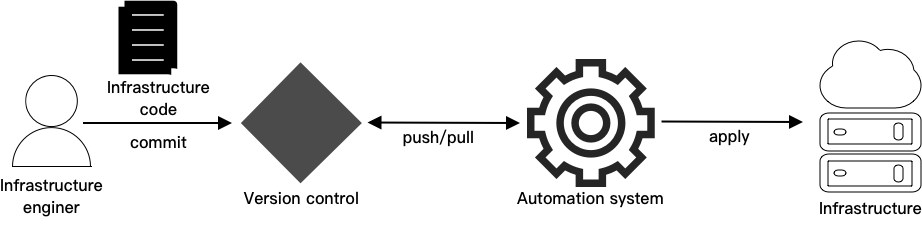
\includegraphics[width= 1\textwidth]{pics/IaC.png}\\
  \caption{基础设施即代码的工作流程}\label{fig:IaC}
\end{figure}

在一个典型的基础设施即代码的工作流程中,如图\ref{fig:IaC}所示,为了进行一次变更,基础设施工程师会在一个包含基础设施代码的文件中表达这个变更。与应用程序代码类似,该代码可以被提交到版本控制系统的存储库中。之后,代码被推送到自动化系统或由自动化系统拉出,随后自动化系统使用该文件和平台特定的集成功能,以便在基础设施中应用所描述的变更\cite{whatisiac}。

\subsection{核心做法}

基础设施即代码的方法囊括了受软件开发启发的若干惯例做法。本节将介绍在本文中被认为是基础的三种惯例做法:定义文件、自文档和版本控制,并讨论它们的好处。

\subsubsection{定义文件}

使用定义文件来描述基础设施是基础设施即代码的核心。按照更传统的方法,基础设施资源通常是用自动化系统的图形界面来定义,并存储在其数据库中,或者根本没有严格的定义,只是在图表和规范文件中记录。按照基础设施即代码的方法,基础设施的所有方面和资源都被定义为代码,也就是文本文件\cite{morris2016infrastructure}。

使用定义文件有几个好处。首先,它们允许精确和详细地描述基础设施资源。此外,对定义的修改可以通过一个文本编辑器来完成,这通常比使用图形界面更快、更简单。最后,定义文件有助于使基础设施更加一致和可重复使用,因为文本定义可以通过最小的调整来复制以适应新的使用情况。另外,根据所使用的IaC工具和语言,可以使用更高层次的编程结构,如模板和函数,以进一步简化这一过程\cite{morris2016infrastructure}\cite{whatisiac}。定义文件的使用直接促成了其余两种惯例做法。

\subsubsection{自文档}

自文档可以被认为是一种惯例做法,也是使用基础设施即代码和定义文件可以得到的直接好处。在传统的方法中,变化的实施和文档是两个独立的过程。这往往会导致文档过时或不存在,因为随着频繁的变化,要保持文档的更新是一个挑战。通过使用精确和详细的代码在定义文件中定义基础设施,代码和文件会自动触发相应行为,并可作为基础设施的文档\cite{morris2016infrastructure}\cite{whatisiac}。

\subsubsection{版本控制}

使用代码和文件来描述基础设施,是软件工程中最广泛使用的做法之一,即版本控制,能够被用于基础设施。使用像Git这样的版本控制系统(VCS),代码可以在代码仓库中进行组织和版本管理。对代码所做的每一个改动都必须提交到版本控制系统中,版本控制系统会跟踪所有改动的历史,并支持在历史的不同点上查看代码库的不同状态(快照)。因此,代码仓库可以作为代码的可信来源。

这可以为基础设施代码服务。首先,对所有基础设施的定义有一个单一的可信来源,可以改善协作和变化的一般可见性,因为历史日志可以作为一个易于使用的时序的变化描述。此外,这也允许可追溯性和可审计性,因为每一个变更都可以追溯到VCS中的提交,而提交中通常都有关于做出变更的人的信息,也有关于变更的描述或理由。最后,历史日志和VCS的操作也可以在回滚时有所帮助,基础设施可以恢复到一些经过测试的安全状态。

\subsection{工具和范式}

为了根据定义文件正确和有效地管理实际的基础设施,需要自动化工具或系统。本节介绍基础设施即代码工具的概况,并讨论了所使用的两种主要编程范式。

\subsubsection{工具类型}
目前IaC和相关工具的前景相当广阔,我们可以将它们大致分为以下四类\cite{whatisiac}。

\paragraph{脚本工具}

使用常见的操作系统脚本工具和语言,如Bash、Powershell、Python、Perl等,是使用代码管理基础设施的最简单方法。虽然它们足以完成简单的任务,但这些工具在更复杂的情况下不能很好地扩展。这些工具本质上使用的是指令式的方法。

\paragraph{配置惯例系统}

配置惯例系统是一套功能更全面的系统,如Chef、Puppet或Ansible,它们通常用于以通用方式管理服务器。这些工具倾向于使用标准或专门的远程连接协议和代理与服务器直接通信,以便对软件进行安装和配置。一般来说,这类工具倾向于使用特定的概念和术语,指令式和声明式的工具都可以找到。

\paragraph{配置(provisioning)工具}

这类工具通常提供更高层次的抽象,允许用户创建、修改和删除动态基础设施平台的资源。其中最知名的例子是AWS CloudFormation和Terraform。两者都采用声明式方法,其中CloudFormation使用JSON,Terraform使用自定义的、特定领域的配置语言(DSL)来定义文件。CloudFormation是专门针对AWS平台的,而Terraform则可以在许多不同的平台上使用,因为它可以通过定制的供应商来扩展,几乎可以用于任何符合动态基础设施要求的平台。另外,大多数动态平台也以命令行工具或软件库的形式提供指令式配置工具,如AWS或Google SDK。

\paragraph{基于容器的编排系统}

基于容器的编排系统通常是以IaC原则设计的全动态基础设施平台。这方面的例子有Docker Swarm、Kubernetes、Nomad等等。其核心是提供一个基础设施级别的抽象,如计算、存储和网络。然而,容器的内在特征使IaC成为可能。容器封装了单个应用环境的全部内容,可以用代码(如Dockerfile)来定义,并打包成一个不可变的镜像。此外,容器编排系统(如Kubernetes、Nomad)通过允许系统中的所有资源被声明性地定义,进一步拥抱IaC。

\subsubsection{指令式和声明式}

IaC工具和系统通常使用两种主要的编程范式:指令式和声明式。

使用指令式范式(如脚本或Chef),定义文件中的代码本质上是一组指令,按照特定的顺序执行,以达到基础设施的期望状态。换句话说,指令式用户不仅要求用户描述所需的基础设施资源,而且至少在某种程度上还要求用户描述如何以及以何种顺序应用配置。

使用声明式方法,代码更简单,专门用于定义资源对象、列表和层次结构。在这种情况下,用户不需要知道在一个特定的平台上应该如何配置资源,甚至往往不需要知道以何种顺序配置。这些问题被抽象出来,委托给IaC工具本身。

这两种风格都有优点和缺点。为了强调要执行的单个指令,指令式范式可以被认为是一种更强大的方法,可以支持最复杂的特殊配置。另一方面,声明式方法不那么强大,而且通常受到所用IaC系统能力的限制。然而,从用户的角度来看,声明式编写的文件提供了更简单的读写体验,因为它不要求用户对如何改变基础设施有专业的知识。此外,它们还允许更快地发现和分析基础设施(文件)的不同状态之间的差异,并减少了工作量。

指令式工具使用时拥有许多专门的和不一致的配置,更像是把基础设施当作``宠物''而不是``牛'',使管理更具挑战性和不可扩展性,这种情况应该尽可能避免。这使得指令式工具的价值主张与声明式工具相比要逊色得多,声明式工具欢迎``牛''的方式,并促进标准化、一致性和可重复使用。

\section{状态调谐}\label{section:reconciliation}

在这一节中,我们将探讨一种在大多数声明式IaC工具和系统中常见的模式,并从一般的角度讨论其变化和用途。这种模式被称为状态(state)调谐。

\subsection{从实际状态到期望状态}

声明式IaC工具的基本特征之一是能够接受对期望状态(如特定的基础设施资源集)的描述,并自动变更实际状态(如AWS账户中配置的对象/服务),使其反映期望状态。

\begin{figure}[htbp]
  \centering
  
\includegraphics[width=0.6\textwidth]{pics/simple-state-reconciliation.png}\\
  \caption{状态调谐}\label{fig:ssr}
\end{figure}

图\ref{fig:ssr}中的这种模式就是状态调谐,一般来说,它可以被定义为使目标状态与源状态一致的过程。在本论文中,状态调谐将主要在软件应用程序和基础设施的管理中被考虑,因此,在大多数情况下,目标状态将被视为所需的、用户定义的状态,如IaC,而实际状态将被视为被管理的平台、基础设施或应用的状态。

\subsection{持续状态调谐}\label{section:continus-reconciliation}

在很多情况下,调谐过程是按需触发的(例如,由用户手动触发,或因基础设施代码的新变化而自动触发),并执行一次,直至完成。许多IaC工具,包括Terraform,都采用这种方法。

然而,这种方式有一个缺点,那就是只有在调谐过程结束后,两个状态(期望的和实际的)的一致性才能实现。在任何时候,某些事件,例如绕过IaC的对基础设施进行的手动变更,都可能导致两个状态之间的不一致和漂移。通过这种一次性的方法,导致的不一致直到下一次触发调谐过程时才会被解决,而这可能要到下一次对IaC代码修改时才会发生。

更先进的系统,如Kubernetes中的调谐功能,能够通过不断观察调谐循环中的状态并做出反应,持续尝试确保一致性。这种方法在本论文中被称为持续状态调谐。

\subsubsection{实现技术}

一个基本的实现技术是在定时器的提醒下定期执行一个新的调谐过程。虽然朴素,但这个解决方案是合适的,特别是在变化率较低的环境中。然而,环境中的变化越频繁,为了及时对变化做出反应,核对的时间间隔就需要越短。这可能会在非常短的间隔时间内产生负载和性能影响。

一个改进方法是以基于事件的方式执行调谐过程,每次调谐作为对表明发生变化的事件的反应。例如,如果使用图\ref{fig:IaC}中的IaC工作流,那么期望状态方面的事件可以是版本控制中的一个新变更。此外,调谐系统也需要接收关于基础设施(实际状态)中的资源变化的事件并作出反应。通过对来自双方的事件(期望状态和实际状态)的反应进行调谐,调谐过程只在需要的时候运行,这可以大大改善性能并减少API的负载。

基于事件的方法是否可以实现,取决于实际状态背后的平台,它必须支持产生关于其资源变化的事件。Kubernetes系统原生支持这一点,这是其主要卖点之一。


\section{容器虚拟化技术}
操作系统级的虚拟化,也被称为容器化,是指操作系统的一种功能,其中内核允许存在多个孤立的用户空间实例,这些事例被称为容器。

在容器内运行的程序只能看到容器的资源,即连接的设备,也就是卷;文件和文件夹;网络;容器的操作系统和架构;CPU和内存。看起来容器类似于虚拟机,但是,与虚拟机不同的是,容器化允许应用程序使用与它们运行的系统相同的Linux内核,而不是创建一个完整的虚拟操作系统。在类Unix操作系统上,这个功能可以看作是标准chroot机制的高级实现,它改变了当前运行进程及其子进程的表象根文件夹。

操作系统级的虚拟化在最近几年开始流行,但却是一个老概念。chroot机制是在1979年第七版Unix中发布的。然后,这个功能在FreeBSD Jails中得到了扩展,在2000年3月发布的FreeBSD v4.0中引入。在接下来的9年时间里,FreeBSD Jails增加了CPU和内存限制、磁盘空间和文件数量限制、进程限制以及多IP的网络等功能。2001年,Linux-VServer被发布用来创建VPS(虚拟私人服务器)和隔离的虚拟主机空间。

在2013年美国PyCon大会上,Solomon Hykes提出了Docker是容器的未来。Docker是一个基于Linux的平台,通过基于容器的虚拟化来开发、运输和运行应用程序。和前面介绍的系统一样,它利用主机的操作系统内核来运行多个隔离的用户空间实例,在Docker中这些实例被称为容器。Docker发展很快,迅速成为云容器化的事实标准\cite{cloudcontainertech}。

在Docker发布仅7个月后,Docker和红帽宣布重大合作,包括兼容Fedora/RHEL,并开始在红帽OpenShift内使用Docker作为容器标准\cite{dockerredhat}。次年Kubernetes诞生,并在2015年被采用为完全重新设计的OpenShift 3.0的基础\cite{openshiftk8s}。

\section{Kubernetes}

Kubernetes在很大程度上利用了\ref{section:reconciliation}节中定义的状态调谐模式。本节介绍并进一步深入Kubernetes,描述它的架构,它对状态调谐的使用,最重要的是它的API可扩展性特征,它可以实现并促进自定义用例的持续状态调谐循环,这也是本论文的部分主题。

正如Kubernetes的文档中所说,它是一个可移植的、可扩展的、开源的平台,用于管理容器化的工作负载和服务。它还指出,该平台促进了声明式配置和自动化\cite{whatisk8s}。在高层次上,Kubernetes作为一个开源的、与供应商无关的平台,以容器的形式托管应用程序和工作负载,这些容器在节点池上被动态地调度。它为网络、存储和其他基础设施层面的问题提供了抽象,并为配置外部资源(如负载均衡器或云中的块存储)提供了集成。

Kubernetes的诞生源于Google内部的容器编排工具Borg,Google在2014年6月\cite{googleopen}将其开源\cite{k8sorigin}。虽然Borg是用C++编写的,但Kubernetes是用Go实现的,Go是谷歌设计的一种静态类型化、编译的编程语言。因此,Go是大部分Kubernetes相关项目的语言,包括Operators。


\subsection{Kubernetes集群架构}
即使Kubernetes可以运行在单个物理节点上,例如Kubernetes Minikube和OpenShift CloudReady Containers允许在本地运行单节点Kubernetes,但它通常是运行在多个主机的集群上。

图\ref{fig:k8s-arch}所示为Kubernetes架构,由一组相对较小的服务组成,它们主要通过向一个共同的元数据库读写数据进行合作和交流。在一个典型的集群中,有两组节点:建立控制平面集群的主节点和实际运行应用程序的工作节点。

在此基础上,服务可以进一步分成两组:控制平面组件和节点组件。在大多数配置中,控制平面组件只驻留在主节点上,而节点组件是通用的,驻留在所有的节点上\cite{k8scomponents}。

\begin{figure}[htbp]
  \centering
  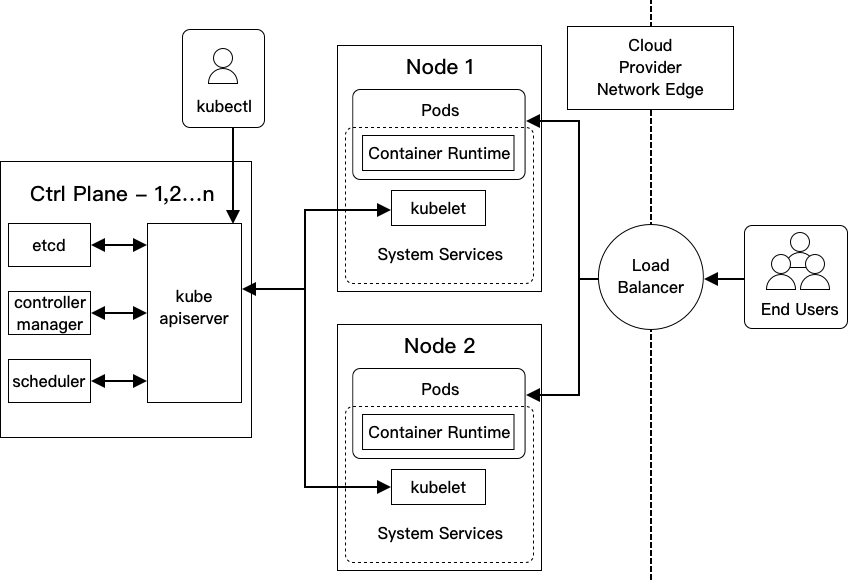
\includegraphics[width=0.85\textwidth]{pics/Kubernetes-architecture.png}\\
  \caption{Kubernetes架构图}\label{fig:k8s-arch}
\end{figure}

\subsubsection{Kubernetes控制面}
如图\ref{fig:k8s-ctrl}所示,Kubernetes控制面由运行在主节点上的各种组件组成。与本文工作相关的主要有以下几个组件:

\paragraph{etcd(元数据库)}

etcd对于Kubernetes跨节点工作至关重要,因为它提供了一个轻量级和分布式的键值存储,可以跨越多个节点。Kubernetes使用etcd来存储配置数据,这些数据可以被集群中的每个节点访问。它存储了Kubernetes的所有配置与状态相关的数据,是系统的核心。

\paragraph{kube-apiserver}
kube-apiserver是整个集群的主要控制模块。etcd负责可靠地存储所有的元数据,但组件并不直接操作这些数据,而是由kube-apiserver提供便利。这个组件作为etcd之上的一层,承载着Kubernetes API,所有的管理工具,包括Kubernetes命令行工具kubectl,都是通过它暴露的那些API与Kubernetes进行通信的。 kubectl是默认的从本地计算机与Kubernetes集群交互的方法,允许管理集群、部署及管理Kubernetes对象。``kubectl apply''是最常用的部署命令。


\begin{figure}[htbp]
  \centering
  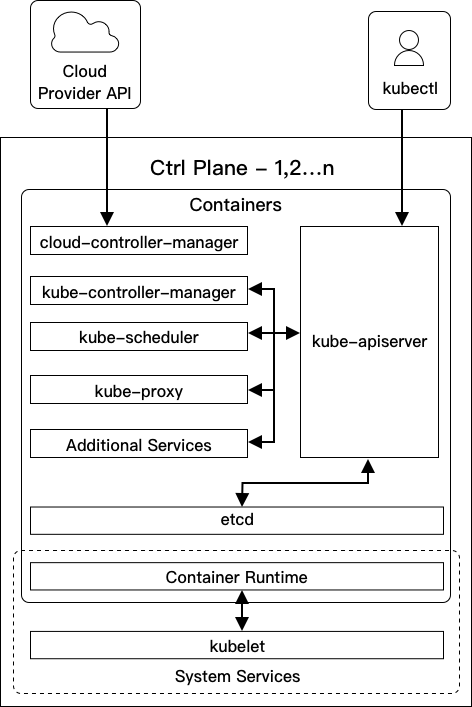
\includegraphics[width= 0.5\textwidth]{pics/K8s-ctrl-plane.png}\\
  \caption{Kubernetes控制面\cite{gorillaguide}}\label{fig:k8s-ctrl}
\end{figure}


\paragraph{kube-controller-manager}
kube-controller-manager是一个具有许多职责的通用服务,可以将其视为控制器组件的集合。这其中的每一个控制器都会调节集群的状态,管理工作负载生命周期,或者执行常规任务\cite{gorillaguide}。

当检测到一个变化时,控制器读取新的信息并执行满足所需状态的程序。这可能涉及到扩大或缩小应用程序的规模,调整端点等。例如,ReplicaSet确保为一个应用程序定义的副本数量与当前部署在集群上的数量相匹配。这里的每个控制器与用户实现的自定义控制器一样都遵循\ref{section:controller-pattern}的控制器模式。

\subsection{Kubernetes中的状态调谐}

Kubernetes中的大部分组件和功能都是通过\ref{section:reconciliation}节中描述的持续的、基于事件的状态调谐模式的小型应用实现的。本节阐述这种用法,并通过一个使用Kubernetes核心资源类型和组件的例子来说明这一概念。

\subsubsection{控制器模式}\label{section:controller-pattern}

在Kubernetes中,状态调谐的使用被包含在被称为控制器的服务中,其名称基于控制理论中的控制循环的概念,是一个调节系统状态的无限循环\cite{k8scontroller}。

\begin{figure}[htbp]
  \centering
  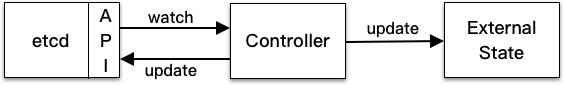
\includegraphics[width= 0.8\textwidth]{pics/controller-pattern.png}\\
  \caption{Kubernetes中的一个控制器}\label{fig:k8s-controller-pattern}
\end{figure}

如图\ref{fig:k8s-controller-pattern}所示,一个控制器通过Kubernetes API不断监视Kubernetes状态中的一些对象的变化。被监视的对象,特别是它们的规格属性,描述了一些期望的状态,控制器将试图在现有环境的相关部分(实际状态)达到这些状态。

换句话说,控制器主持调谐循环,执行如\ref{section:continus-reconciliation}节所定义的持续状态调谐。控制器可以对一个事件做出响应,更新etcd中的一些资源,或更新一些外部环境(如云提供商的资源),或两者都更新。\ref{section:reconciliation}所定义的期望状态和实际状态的划分,在不同的控制器实现和它们被设计用来解决的问题之间是不同的。

\subsection{自定义状态调谐}\label{section:custom-reconciliation}

正如本节所讨论的,状态调谐是Kubernetes的核心,Kubernetes及其API的许多方面和功能都有助于实现调节循环和控制器。基于调谐的持续控制方法代表了一种通用模式,可以用于实现Kubernetes核心功能以外的用例,包括Kubernetes特有的自动化或者扩展,也包括完全自定义的应用。这Kubernetes可扩展性的核心体现,能够实现具有自定义逻辑的调谐循环。

\subsubsection{自定义资源定义(Custom Resource Definitions)}

为了实现自定义调节,有必要用单独的自定义模式(schema)来定义新的自定义资源。在Kubernetes中,这可以通过使用自定义资源定义CRD来完成,CRD是Kubernetes中的一种特殊资源类型(CustomResourceDefinition)。

CustomResourceDefinition类型的资源的结构提供了一些字段,它们被用于指定应添加到Kubernetes API中的自定义资源。一旦提交了有效的CRD,Kubernetes API将自动扩展新的端点,其URL结构取决于一些字段。同样,该资源也将变得可用,可以通过kubectl命令行客户端查询和操作。该资源将自动支持所有Kubernetes API动作。核心字段的意义如下:

\paragraph{API Group}

API Group是一个需要为新的自定义资源指定的属性。API Group的概念被用于大多数Kubernetes资源(除了像Pod这样的核心资源),将相关的资源类型组合在一起,并创建一个Kubernetes API的逻辑``分区''。该组成为API端点的URL的一部分,也是自定义资源元数据的一部分,也可用于权限控制。使用域名来命名API组是很常见的,以表明所有权或作者。

由于CustomResourceDefintion本身也是一种Kubernetes资源,如YAML文件\ref{listing:1}第1行所示,它所属的API Group是apiextensions.k8s.io

\paragraph{Versions}

CRD的规范还需要为新资源指定至少一个版本。版本指定了新资源结构的模式,使用OpenAPI6的模式规范格式。每个版本都可以被启用或禁用,而且其中一个版本必须被配置为存储版本。存储版本代表实际将被存储在etcd中的结构,而其他版本将简单地被转换为存储版本。

\paragraph{Names}

要声明一个新的Kubernetes API资源,需要指定其名称的几种形式。复数名称(YAML文件\ref{listing:1}第12行的universalcontrollers)将被用于Kubernetes API端点的资源的URL结构中,即/apis/universalcontroller.njuics.cn/v1alpha1/universalcontrollers。单数名称(第10行)通常用于kubectl CLI命令,例如,kubectl get universalcontroller。也可以为其定义更短的别名,如YAML文件\ref{listing:1}的第13-15行所示。最后,必须指定的最后一个名称是kind,它是资源类型的名称,在配置清单中使用。

\paragraph{Scope}

CRD还必须指定新资源的范围。一般来说,在Kubernetes中,一个特定的资源类型可以是命名空间范围的,即每个对象必须属于某个命名空间,或者是集群范围的,即每个对象是全局的。在CRD中,这是用范围参数指定的,如YAML文件\ref{listing:1}的第17行。

\subsubsection{自定义控制器}

一旦新的CRD被注册,各自的自定义资源对象及其规格就可以被应用到Kubernetes。虽然这允许声明和存储所需的状态,但需要有一个自定义控制器,以便将规范应用到真实的状态或环境中。自定义控制器需要使用watch API去监听这个新资源对象的相关事件,并对事件作出响应行为。

自定义控制器不是Kubernetes的一部分,需要单独安装。由于所有的逻辑和依赖都包含在控制器的代码中,安装可以通过简单地在容器中部署控制器来完成,使用与其他应用程序相同的方法,如添加一个新的Pod或一个Deployment(一组副本Pod)对象。

\subsection{Operator模式}

\ref{section:custom-reconciliation}节描述的方法通常被称为Operator模式。这个术语基本上是指将控制器模式(\ref{section:controller-pattern}节)应用于一些定制的、特定领域的用例。遵循这种模式的服务被称为Operator,并与一个CRD配对。

Kubernetes官方文档将Operators描述为``Kubernetes的软件扩展,利用自定义资源来管理应用程序及其组件''\cite{k8soperator}。一个Operator本质上就是一个自定义资源类型和一个监视该资源类型并做出实际操作的自定义控制器的组合。控制器是Kubernetes中的一个核心概念,它被实现为一个控制循环,在Kubernetes中的一个Pod内持续运行,它比较对象的期望状态和当前状态,并在需要时随时调和这种状态。事实上,当对象的当前状态与期望状态不同时,负责管理的Kubernetes Operator会对对象发出指令,使其最终达到期望状态。下面介绍一些开发者实现Operators所使用的主要工具。

\subsubsection{主要的开发工具}\label{section:wayofimplement}

\paragraph{client-go}


\begin{figure}[htbp]
  \centering
  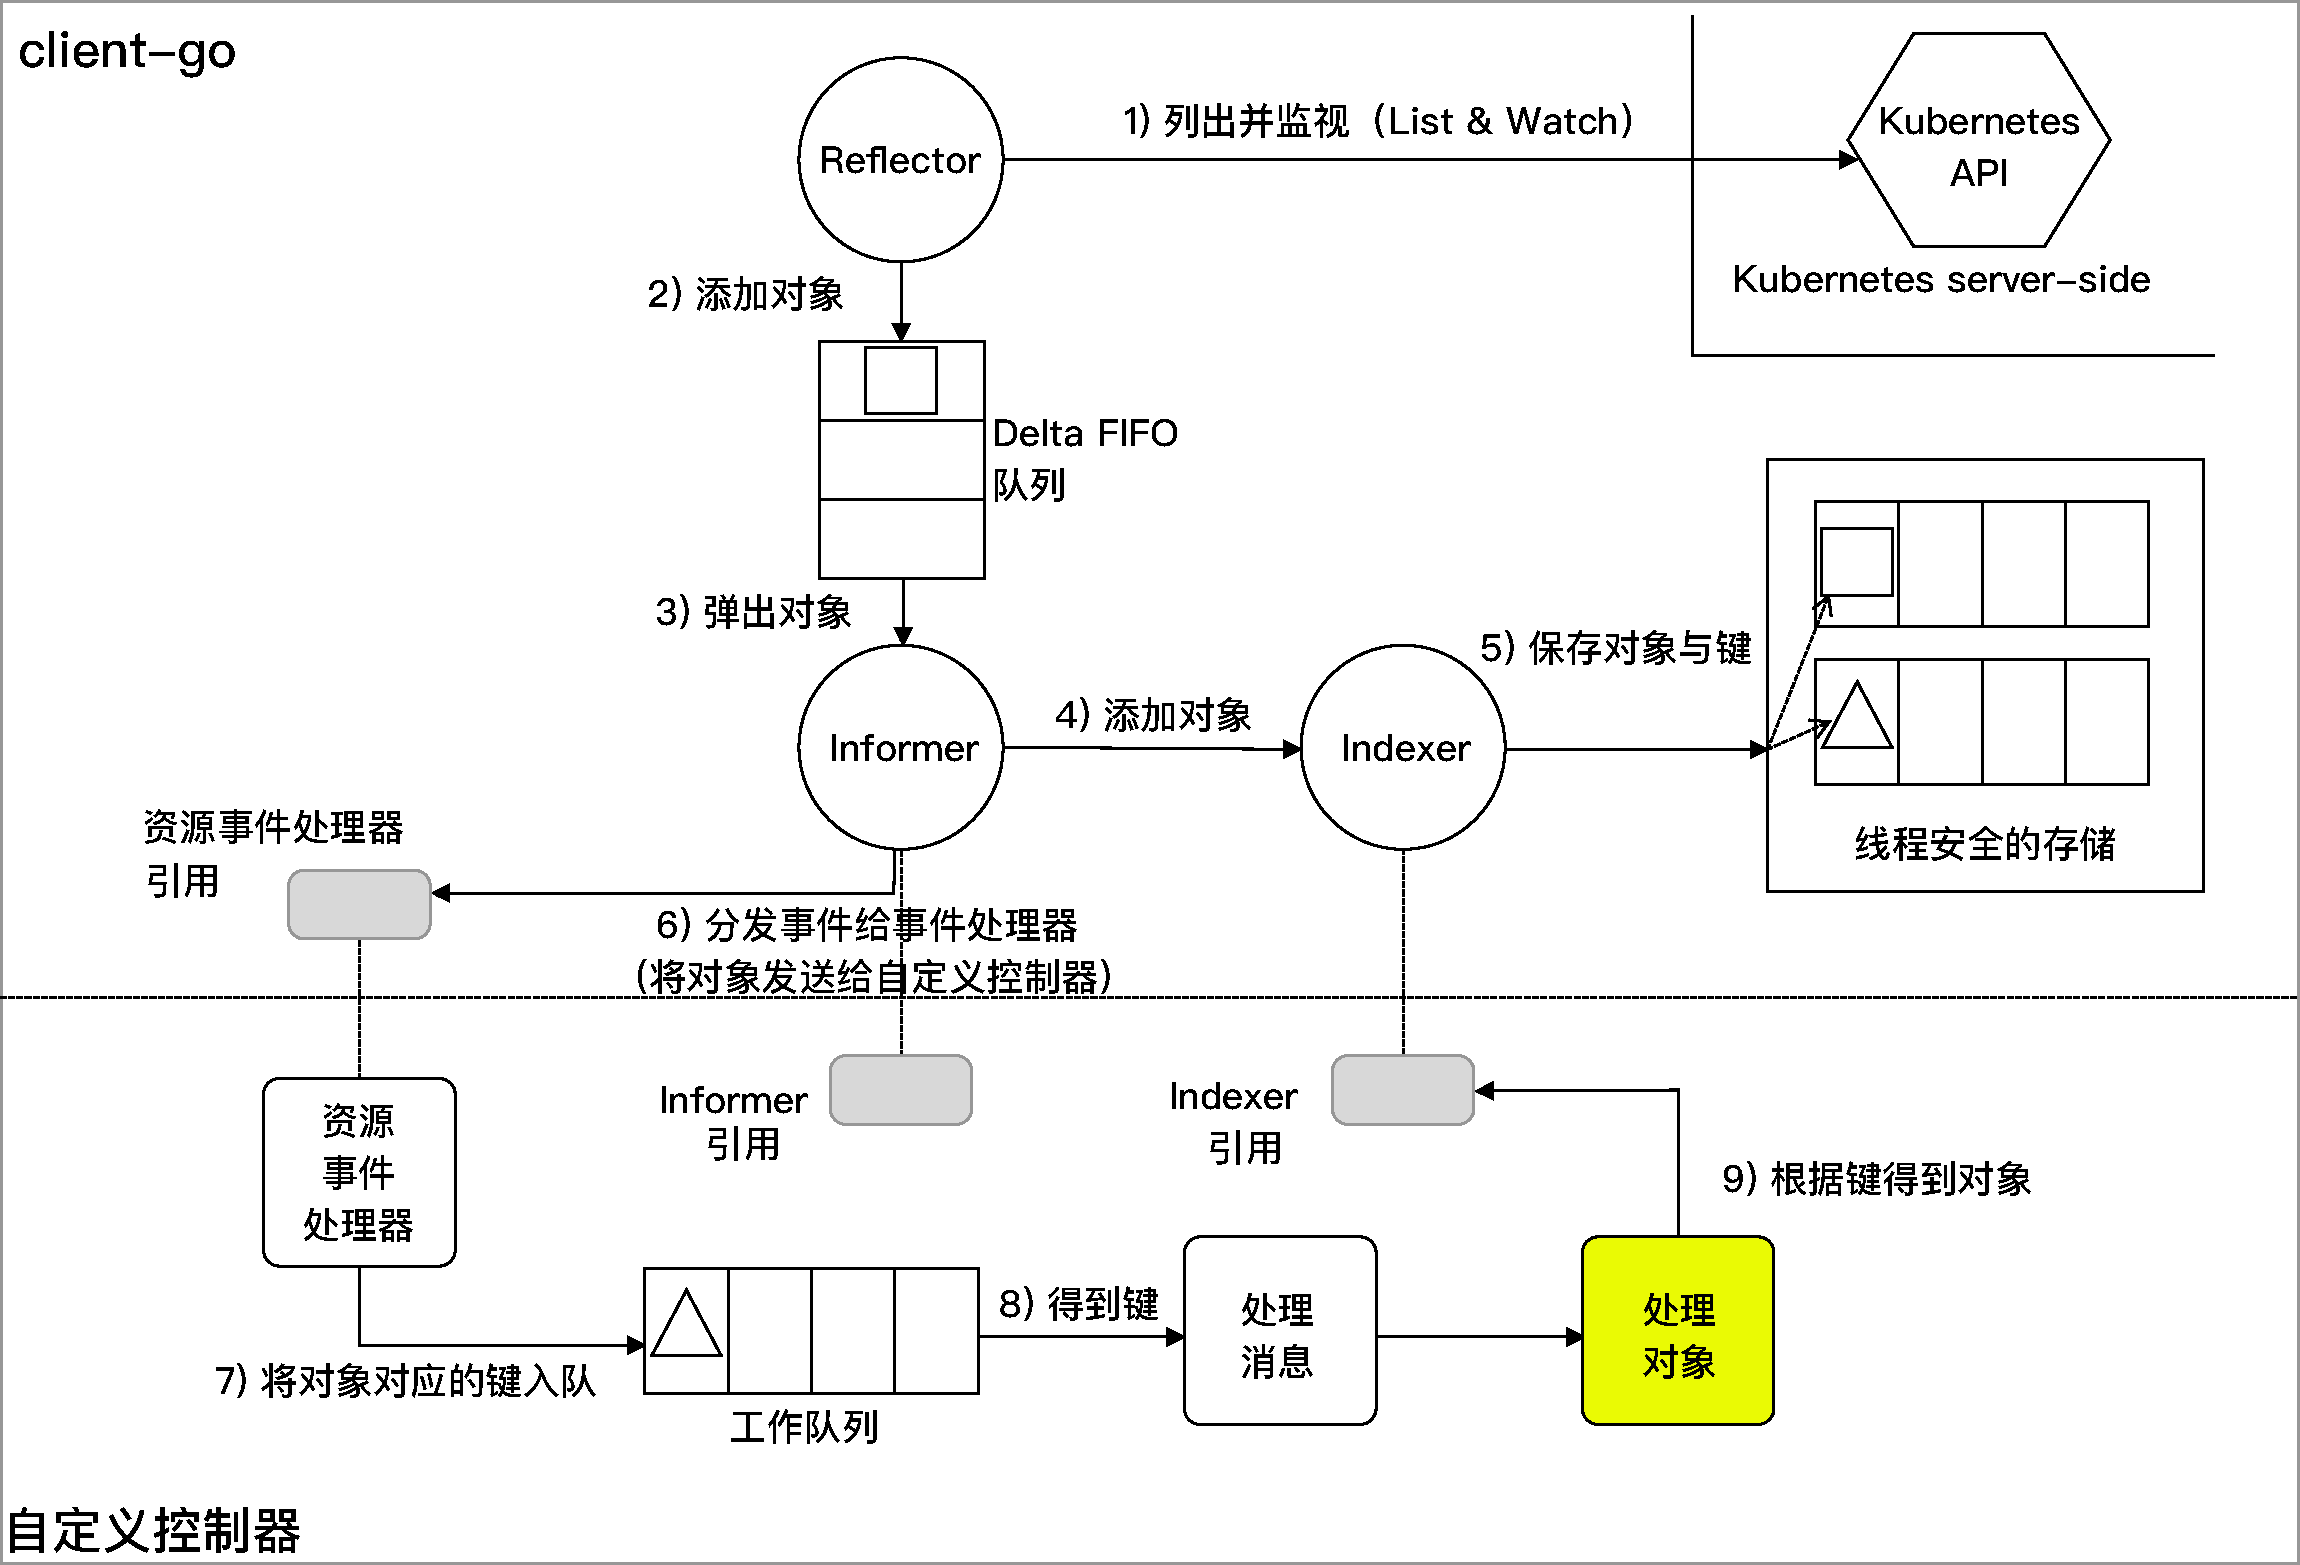
\includegraphics[width= 1\textwidth]{pics/client-go-controller-interaction.pdf}\\
  \caption{控制器工作方式}\label{fig:client-go-controller-interaction}
\end{figure}

client-go是最成熟的Kubernetes客户端库,它和Kubernetes自身一样都由Go语言编写而成,是Kubernetes官方第一个提供的客户端库,而且正在被Kubernetes本身的组件内部使用,这也意味着它是经过良好测试和可靠的\cite{controllerclientgo}。

该库封装了几个抽象和较小的包,便于实现Kubernetes的集成和与Kubernetes API的通信。有三个包与基本的Kubernetes API通信有关\cite{controllerclientgo}:

\begin{itemize}
	\item kubernetes包,提供静态(和静态类型)的客户端,可用于对Kubernetes API执行涉及Kubernetes原生资源类型的操作。
	\item dynamic包,它提供了一个动态客户端,能够对任何资源类型(原生和自定义)进行通用操作。
	\item transport包,在与Kubernetes通信时帮助处理低级别的传输细节,如使用有效的认证建立连接等。
\end{itemize}

此外,由于client-go在整个Kubernetes代码库中被使用,包括复杂的场景,它还附带了额外的工具、实用程序、对象和抽象,以简化Kubernetes集成。

鉴于本文的主题与状态调谐和自定义Kubernetes控制器有关,客户端最引人注目的功能是Informer模式的实现\cite{informer}。

Informer是对Kubernetes API的实时观察功能的抽象,API可以将集群中任何对象的任何变化事件通知消费者。它们提供了一个接口,允许开发者为特定的Kubernetes资源类型有效地建立所述的变化流连接\cite{informer}。这代表了实现自定义控制器的关键功能,它需要不断监视和应对资源相关变化的。

图\ref{fig:client-go-controller-interaction}展示了使用clieng-go编写的控制器的工作方式。首先介绍一下client-go提供给开发者的组件:
\begin{enumerate}
	\item \textbf{反射器(Reflector)}:反射器监视着Kubernetes API中的指定资源类型(Kind)。完成这项工作的方法(function)是``ListAndWatch''。监视的对象可以是内置的原生资源,也可以是自定义资源。当反射器通过监视API收到有新资源诞生的通知时,它使用相应的listing API获得该对象,调用``watchHandler''方法,将其放入``Delta FIFO''队列中。
	\item \textbf{通知器(Informer)}:通知器从``Delta FIFO''队列中弹出对象。它的工作是保存对象以便以后检索,并向自定义控制器传递对象。
	\item \textbf{索引器(Indexer)}:索引器提供索引对象的功能。一个典型的索引用例是基于对象标签创建索引。索引器可以基于几个索引功能来维护索引。索引器使用一个线程安全的数据存储来存储对象和它们的键。默认会使用Store类型中一个名为MetaNamespaceKeyFunc的方法来生成键,该方法将一个对象的键生成为该对象的<命名空间>/<名称>组合。
\end{enumerate}

而自定义控制器中有以下组件:
\begin{enumerate}
	\item \textbf{资源事件处理器(Resource Event Handlers)}:资源事件处理器是回调函数,当通知器(Informer)向控制器传递一个对象时,它将被调用。编写这些函数的典型模式是获取被传递对象的键,并将该键排入工作队列(workqueue)等待进一步的处理。
	\item \textbf{工作队列(Workqueue)}:工作队列将对象的传递与处理脱钩,接受到对象后不会立即处理而是放入队列中。
	\item \textbf{处理程序(Process Item)}:处理程序被用于处理工作队列中的项目,它通常使用索引器来检索与键对应的对象。
\end{enumerate}

\paragraph{controller-runtime}

controller-runtime建立在client-go库之上,用构建控制器的相关概念和API来扩展它,其中包括\cite{k8s-sigs}读写Kubernetes对象的高级客户端、用于高效获取Kubernetes对象的缓存、用于共享依赖关系和启动控制器的管理器(Manager)、核心抽象控制器、用于扩展Kubernetes API的对象准入流程的Webhook、由事件触发执行的调谐器、封装Kubernetes事件流的源。



\section{小结}
本章主要介绍了声明式的通用Kubernetes Operator设计到的相关技术和场景。首先介绍了动态基础设施及其标准。之后解释IaC的概念,并描述了相关的实践和有点,介绍了支持这些实践的不同类型的工具,并在IaC的背景下讨论了指令式和声明式编程范式。接着介绍IaC的核心机制之一状态调谐,最后深入研究了Kubernetes平台的细节,描述了它如何拥抱声明式并且使用持续调谐循环。

%%%%%%%%%%%%%%%%%%%%%%%%%%%%%%%%%%%%%%%%%%%%%%%%%%%%%%%%%%%%%%%%%%%%%%%%%%%%%%%
\chapter{声明式的通用调谐技术}\label{chapter_framework}
本文所陈述的声明式的通用Kubernetes Operator,即UniversalController,实现了声明式的通用调谐技术,主要是为了让开发者更容易的去实现以及部署Kubernetes Operators,进而扩展Kubernetes的API,而实现这一点的核心就是声明式调谐技术。

\section{现有的Kubernetes Operators实现方式}

Kubernetes的Operator可以简单解释为自定义资源与自定义控制器的组合。自定义资源通过Kubernetes的CustomResourceDefinition机制可以很容易地生成,而自定义控制器需要用户自行编写。

编写自定义控制器是编写代码来管理一个应用程序的生命周期的过程。它需要付出极大的努力,但对各种特殊的要求有最大的自由。这种方法最好用于需要非常特殊功能的应用程序的操作。

开发一个自定义的控制器需要很多对Kubernetes的深入知识,而它们通常对大多数应用程序的生命周期管理是不需要的。除了应用程序生命周期的具体要求外,它还会给开发者带来管理负担,包括测试、升级、改变Operator的存储数据和改变API\cite{kudovscc}。

\subsection{Kubernetes Clients}

在开发控制器时,最自由的做法是使用现有的Kubernetes客户端,可以是Go、Java、JS/Typescript或其他语言的客户端。这些客户端提供了对Kubernetes APIs的直接和底层的访问,没有任何包装或附加层。

这允许使用任何语言,并且不将任何观点强加给开发者。但是,它要求开发者解决很多已知的问题,并且没有为Kubernetes领域的常见问题提供指导\cite{kudovscc}。

\subsubsection{client-go}


\begin{figure}[htbp]
  \centering
  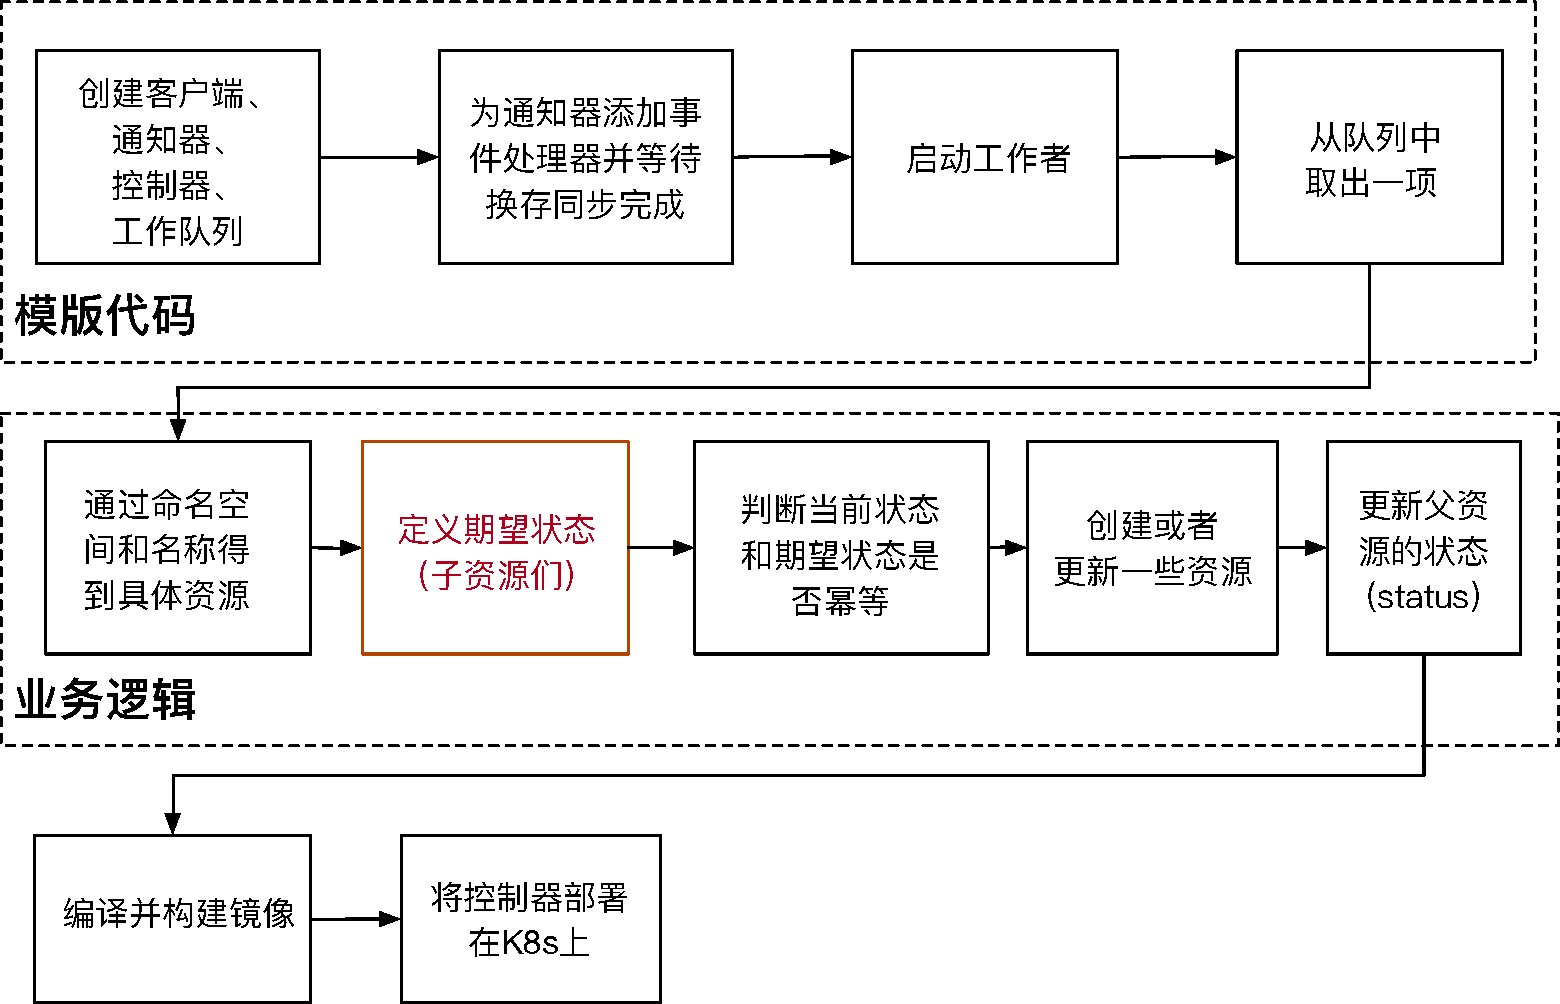
\includegraphics[width= 1\textwidth]{pics/coding-operator.pdf}\\
  \caption{Operator编写流程}\label{fig:coding-operator}
\end{figure}

client-go是最常用也最成熟的客户端库,图\ref{fig:client-go-controller-interaction}描述了控制器的工作方式,图\ref{fig:coding-operator}是使用client-go开发一个自定义控制器的基本流程,除了最后用于部署控制器的两步以外,各个流程都与图\ref{fig:client-go-controller-interaction}中的一个组件或者一个步骤对应。client-go相关代码以模版代码居多,在不同的控制器中,创建客户端、通知器、工作队列的代码都是高度相像的,只是需要处理的资源类型不同。每个控制器真正核心的部分都是``定义期望的状态(子资源们)'',即给出期望状态(state)。

\subsection{Kubernetes Controller Runtime}

正如上一节所讨论的,client-go库提供了许多抽象,可以简化Kubernetes控制器和状态调谐的实现。尽管如此,该库是为了成为一个通用的客户端而设计的,它并没有专门去解决编写控制器的很多问题。

其他项目,如Operator SDK和Kubebuilder,提供了更高层次的抽象。它们专门针对Kubernetes API扩展的开发者,并考虑到自定义控制器的设计。它们都建立在一个共同的核心代码库之上,即controller-runtime\cite{k8s-sigs}。它是一组库,共同代表了用自定义调谐逻辑扩展Kubernetes的通用模型\cite{controllerruntimedoc}\cite{k8s-sigs}。


借助controller-runtime以及代码生成工具,我们可以省去很多模版代码的编写,但是我们依然必须用Go语言来开发Operator项目,依然需要与Kubernetes的API打交道,需要自行处理更新策略,而且也不能规避所有的模版代码,判断实际状态和期望状态是否幂等、对资源进行创建或者更新依然是一套惯例代码样式。

\subsection{问题分析}

在开发Kubernetes Operator时,开发者最关心也是最核心的部分就是调谐逻辑,但是为了实现一个完整的Operator,开发者不得不把大量的精力放在编写一些模版代码或者使用代码生成工具上,而且Kubernetes Operator的成熟开发工具都是用Go编写的,也是为Go项目服务的,对使用其他编程语言的开发者极不友好。而为了使用这些工具,用户也必须去学习Kubernetes API相关的深度知识,进而拉高了门槛。

本文的目的是简化Kubernetes Operators的开发、部署和管理,而通过声明式的通用调谐技术就能很好的做到这一点,接下来开始介绍。


\section{声明式的通用调谐技术}

声明式的通用调谐技术的初衷十分简单,既然开发者实际只关心调谐逻辑,而其他与Kubernetes相关的代码基本都是模版代码或者有惯例可循,那么完全可以将这部分代码代码单独抽取出来,提供一个接口供用户实现,其他的代码都由系统或者框架代劳。基于这个想法实现的就是UniversalController,一个声明式的通用Kubernetes Operator,它实现了通用的资源监视、当前状态与期望状态对比、资源更新等功能,提供声明式的接口,帮助用户通过声明式编程实现Operator,减少了重复工作。

UniversalController自身也是一个Kubernetes Operator,负责监视UniversalController CRD(下文简称UC CRD)并维护它们对应的自定义控制器。UC CRD是对一个自定义控制器的抽象描述。创建一个新的UC CRD等同于在系统中注册一个新的自定义控制器,UC Controller会通过调谐循环维护它。Kubernetes提供的动态API注册机制CustomResourceDefinition,这让用户可以声明式地创建一种新的自定义资源,UniversalController扩展了Kubernetes的API,UC CRD接口进一步让用户可以声明式地创建自定义控制器。借助UniversalController,一个Operator的开发会简化成如图\ref{fig:uc-coding-operator}所示。图\ref{fig:uc-coding-operator}中的Kubeless是一个serverless工具,主要用于将一个函数部署成一个网络服务。

\begin{figure}[htbp]
  \centering
  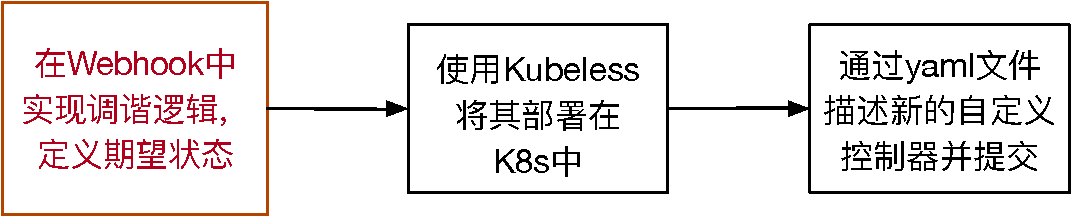
\includegraphics[width=0.8\textwidth]{pics/uc-coding-operator.pdf}\\
  \caption{借助UC实现一个Operator}\label{fig:uc-coding-operator}
\end{figure}


\subsection{自定义资源}

UC CRD是UniversalController提供的声明式API,通过Kubernetes CustomResourceDefinition注册在Kubernetes API中。通过创建一个UC资源,可以很方便的定制一种控制器,它根据父对象中指定的期望状态管理一组子对象,这也是最常见的控制器类型。像Deployment、StatefulSet、TFJob、PytorchJob的控制器都是符合这种模式的。

UC CRD是对控制器的高级抽象,包含了一个控制器运行时需要知道的各项信息,例如事件配置、更新策略和调谐接口访问地址。用户只需要填写好各项字段就能声明式地创建想要的控制器。通过UC CRD实现了以下功能:

\begin{enumerate}
	\item \textbf{声明式的监视(watch)}:用户只需要填写好parentResource对象和childResources对象数组,UniversalController就会对这些资源进行监视,订阅它们的相关事件。
	\item \textbf{声明式的更新策略}:childResources对象数组中的每个childResource对象都有一个updateStrategy对象,通过设置它实现声明式的更新策略,支持OnDelete, Recreate, InPlace, RollingRecreate, RollingInPlace。
	\item \textbf{声明式的调谐}:调谐接口是唯一需要用户编码实现的模块,用户在这里只需要关心实际业务逻辑,开发完成后将其部署成一个web服务,将服务地址填入UC CRD的相应字段即可。用户在编码过程中只需要描述期望的状态即可,而不需要给出具体操作以达到期望状态,这个过程本质上也是声明式的。
\end{enumerate}

\subsection{声明式的监视}

借助UC,开发者不再需要为想监视的每一种类型的资源编写模板代码,而只要简单地列出这些资源的声明。YAML段\ref{listing:declarative-watch}是\ref{section:sample-controller}节的YAML文件\ref{listing:sample-controller-config}的第7到12行,说明该自定义控制器的父资源是Foo(foos是Foo在K8s中的复数表达),子资源是Deployment(deployments是Deployment在K8s中的复数表达)。UC会负责建立监视流(watch stream),这些监视流被所有使用UC创建的控制器共享。开发者可以在UC之上创建任意多的自定义控制器来观察Pod,而kube-apiserver只需要发送一个Pod监视流。UC就像一个解复用器,确定哪些控制器会关注流中的特定事件,并根据需要触发它们的事件处理器(一个函数)。
\begin{lstlisting}[language=yaml,caption=声明式的监视,label=listing:declarative-watch]
parentResource:
  apiVersion: njuics.cn/v1alpha1
  resource: foos
childResources:
- apiVersion: apps/v1
  resource: deployments
\end{lstlisting}

而如果用client-go来编写,需要先创建通知器工厂,再用工厂创建通知器,最后添加事件处理器,对资源的增加、更新、删除做出反应,如代码段\ref{listing:watch-foo-deploy}所示。代码段\ref{listing:watch-foo-deploy}的第5到10行的意思是,对于Foo资源,它的增加、更新和删除触发的事件处理器的工作都是把相关Foo资源的键加入工作队列等待处理,这是对父资源处理的一般惯例。对于Deployment资源,它的增加、更新和删除触发的事件处理器都调用handleObject方法。handleObject的简化版是代码段\ref{listing:watch-foo-deploy}的第22到27行,意思是根据Deployment的OwnerReference信息得到它的父资源Foo的命名空间和名称以定位,将这个父资源的键加入工作队列。这是对子资源处理的一般惯例。代码段\ref{listing:watch-foo-deploy}是典型的模版代码,不同的控制器都遵循这样的惯例,只是资源类型不同而已。
\begin{lstlisting}[language=Go,caption=sample-controller中监视Foo和Deployment的代码段,label=listing:watch-foo-deploy]
kubeInformerFactory := kubeinformers.NewSharedInformerFactory(kubeClient, time.Second*30)
exampleInformerFactory := informers.NewSharedInformerFactory(exampleClient, time.Second*30)
fooInformer := exampleInformerFactory.Samplecontroller().V1alpha1().Foos()
deploymentInformer := kubeInformerFactory.Apps().V1().Deployments()
fooInformer.Informer().AddEventHandler(cache.ResourceEventHandlerFuncs{
	AddFunc: controller.enqueueFoo,
	UpdateFunc: func(old, new interface{}) {
		controller.enqueueFoo(new)
	},
	DeleteFunc: controller.enqueueFoo,
})
deploymentInformer.Informer().AddEventHandler(cache.ResourceEventHandlerFuncs{
	AddFunc: controller.handleObject,
	UpdateFunc: func(old, new interface{}) {
		newDepl := new.(*appsv1.Deployment)
		oldDepl := old.(*appsv1.Deployment)
		if newDepl.ResourceVersion == oldDepl.ResourceVersion { return }
		controller.handleObject(new)
	},
	DeleteFunc: controller.handleObject,
})
func (c *Controller) handleObject(obj interface{}) {
	if ownerRef := metav1.GetControllerOf(object); ownerRef != nil {
		if ownerRef.Kind != "Foo" { return }
		foo, err := c.foosLister.Foos(object.GetNamespace()).Get(ownerRef.Name)
		if err != nil { return }
		c.enqueueFoo(foo)
		return
	}
}
\end{lstlisting}

代码段\ref{listing:watch-foo-deploy-cr}借助controller-runtime库设置监视(watch)。借助controller-runtime提供的高级接口,相比代码段\ref{listing:watch-foo-deploy}要精简的多。但依然要比YAML文件片段\ref{listing:declarative-watch}复杂,还要考虑到Go语言和controller-runtime接口的学习成本,所以使用依旧比较困难。
\begin{lstlisting}[language=Go,caption=controller-runtime版sample-controller中监视Foo和Deployment的代码段,label=listing:watch-foo-deploy-cr]
c.Watch(&source.Kind{Type: &samplev1alpha1.Foo{}}, &handler.EnqueueRequestForObject{})
subresources := []runtime.Object{
    &appsv1.Deployment{},
}
for _, subresource := range subresources {
    c.Watch(&source.Kind{Type: subresource}, &handler.EnqueueRequestForOwner{
        IsController: true,
        OwnerType:    &samplev1alpha1.Foo{},
    })
}
\end{lstlisting}


\subsection{声明式的通用调谐器}
图\ref{fig:uc-arch}中的``Lambda Hook''模块就是UniversalController中的调谐器,以webhook的形式实现。

调谐器的工作本质上其实就是两个翻译过程:
\begin{enumerate}
	\item 根据集群的当前状态(state)得到资源的状态(status)。
	\item 根据资源的specification对Kubernetes集群进行操作,一般是编排一些Kubernetes原生资源,例如Pods、Services等,来完成某个应用(例如数据库)的部署与维护。
\end{enumerate}

\begin{figure}[htbp]
  \centering
  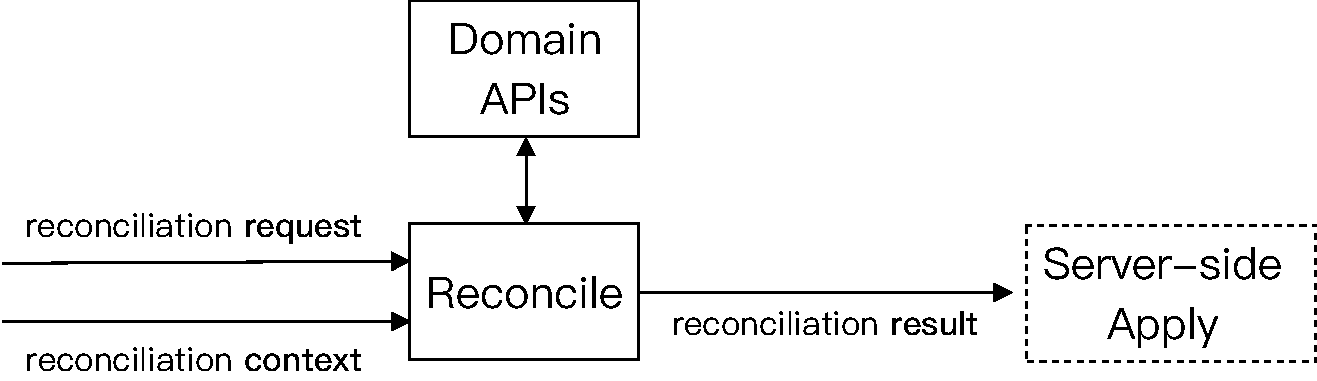
\includegraphics[width= 0.8\textwidth]{pics/reconciler-interface.pdf}\\
  \caption{调谐器}\label{fig:reconciler}
\end{figure}

图\ref{fig:reconciler}是一般的调谐器抽象,它接受调谐请求和当前系统上下文,并返回调谐的结果。在Kubernetes中Domain APIs就是各种资源,包括Pod、Service、ReplicaSet等,用户自定义的资源也包含在其中。在UC中,调谐请求就是当前被处理的资源对象,上下文就是通过标签筛选出的子资源以及相关资源,调谐结果是根据当前状态(state)得到该资源对象的状态(status)以及根据该资源对象的规格(specification)得到的期望子资源。

\begin{figure}[htbp]
  \centering
  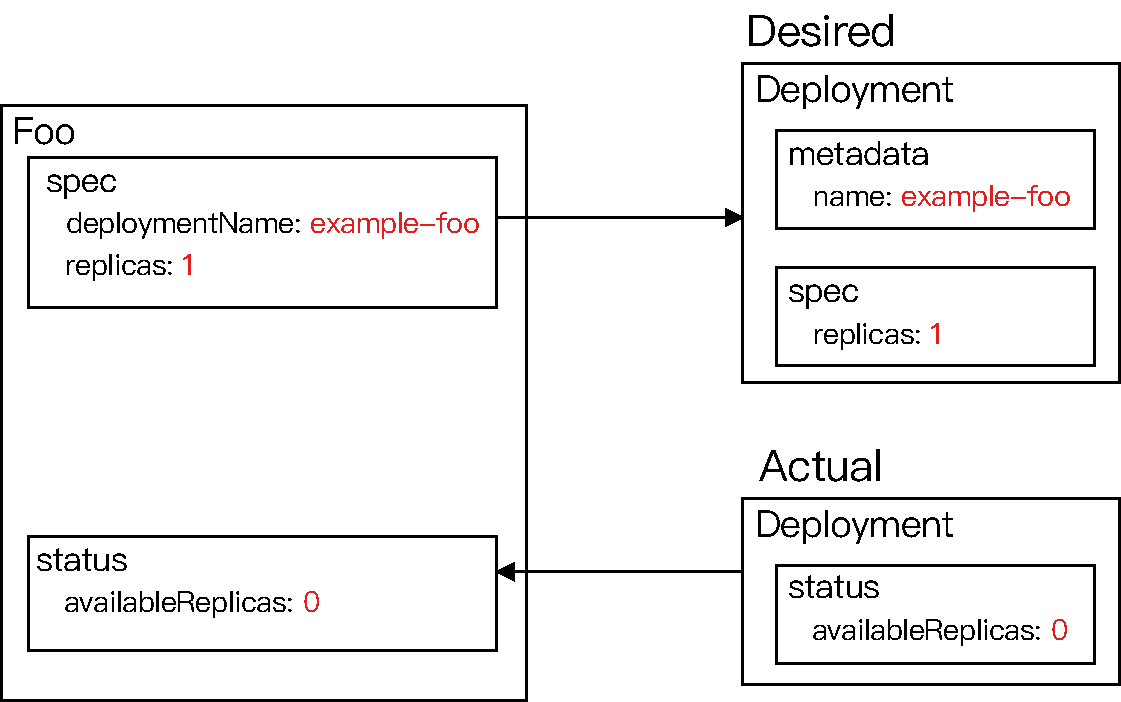
\includegraphics[width=0.8\textwidth]{pics/Foo-reconciliation.pdf}\\
  \caption{sample-controller的调谐过程}\label{fig:Foo-reconciliation}
\end{figure}

举例来说,\ref{section:sample-controller}节的sample-controller负责管理的自定义资源是Foo,它的spec中只有两个字段deploymentName和replicas,代表期望生成的Deployment资源的名称和指定的副本数量,它的status中只有一个字段availableReplicas,代表集群中实际可用的副本数量。图\ref{fig:Foo-reconciliation}展示了sample-controller的一次调谐过程。根据这个Foo的deploymentName和replicas会去生成一个名称为example-foo,副本数量为1的Deployment,这就是第二个翻译过程,对应代码\ref{listing:sample-controller}的第17到41行的desiredDeployment函数。而根据当前集群中实际的Deployment的status中的availableReplicas字段可以得知可用的副本数量此刻为0,所以Foo的status的availableReplicas字段的值也要设置为0,这就是第一个翻译过程,对应代码\ref{listing:sample-controller}的第10到13行。

基于UniversalController编写的调谐器不用去处理资源的增删改查,不用去与Kubernetes交互,只需要去返回期望状态(期望存在的资源集合)。UC Controller会去决定怎么到达期望状态。这个过程与用户直接通过kubectl将资源描述文件提交给kube-apiserver很接近,指令式的操作极少,也是声明式的。

UniversalController使用自己的服务端应用(server-side apply)逻辑,它与``kubectl apply''的逻辑接近,遵循惯例而不是配置。开发者不需要在CRD中提供如何合并旧资源与新资源的提示,自定义资源和原生资源都根据一套``kubectl apply''逻辑得到合并结果。

现阶段调谐器需要以Webhook的形式提供,任何可以编写网络服务并处理JSON的编程语言都可以用于编写这段核心业务逻辑。这是实现语言无关特性的关键。借助serverless工具,开发者实际需要编写的只是一个函数而已,其lambda表达式为(parent, children, related) => \{... return (status, children)\}。例如,\ref{section:sample-controller}节的代码段\ref{listing:sample-controller}中的reconcile就是这样一个函数,最后只要返回调谐结果即可,不需要做任何增删改查之类的指令式操作。而使用client-go或者controller-runtime实现调谐逻辑时,都需要开发者调用接口对资源进行增删改查。代码段\ref{listing:crud-rc}是用client-go编写时增删改查资源相关的代码。第1行获取本次调谐处理的Foo资源对象;第2行获取已经存在的子资源Deployment;第3到5行表示如果子资源还不存在,就创建它;第6到8行表示如果已存在的Deployment的replicas与Foo中的不一致,就更新它;第9行更新Foo的status。
\begin{lstlisting}[language=Go,caption=sample-controller中对资源进行增删改查的代码段,label=listing:crud-rc]
foo, err := c.foosLister.Foos(namespace).Get(name)
deployment, err := c.deploymentsLister.Deployments(foo.Namespace).Get(deploymentName)
if errors.IsNotFound(err) {
    deployment, err = c.kubeclientset.AppsV1().Deployments(foo.Namespace).Create(context.TODO(), newDeployment(foo), metav1.CreateOptions{})
}
if foo.Spec.Replicas != nil && *foo.Spec.Replicas != *deployment.Spec.Replicas {
    deployment, err = c.kubeclientset.AppsV1().Deployments(foo.Namespace).Update(context.TODO(), newDeployment(foo), metav1.UpdateOptions{})
}
_, err := c.sampleclientset.SamplecontrollerV1alpha1().Foos(foo.Namespace).Update(context.TODO(), fooCopy, metav1.UpdateOptions{})
\end{lstlisting}

\subsection{服务端应用(apply)}


\subsection{声明式的更新策略}

一般的Operator在比较期望状态和实际状态后,会对资源进行更新,进行增删改查的操作。而不同的资源适合不同的更新策略,例如Pod一般会用重新创建,因为当一个Pod已经在Kubernetes中存在,它能修改的只有metadata中的标签(labels)和附加说明(annotations),spec中的字段都不能修改,如果需要修改,就只能删除重建。而Deployment除了名字和命名空间都可以修改,直接更新原资源即可。

在借助UC实现的自定义控制器中,UC Controller会代为执行更新相关操作,为了更灵活的进行更新,具体资源具体分析,内置了很多更新策略,通过声明式接口供用户使用。Kubernetes的原生资源Deployment和StatefulSet都有对它们管理的Pod进行滚动更新的功能。UniversalController也支持滚动更新,内置了相关的更新策略,并且可以通过声明式使用,开发者只需要在UC资源中填入相应字段就可以让自己的控制器拥有滚动更新的能力。例如,\ref{section:catset}节中的CatSet用例是在基于UC重写的StatefulSet,为其添加对滚动更新的支持,只需要YAML文件\ref{listing:catset-controller-config}中的第16到21行,也就是YAML片段\ref{listing:declarative-rolling}中的第4到9行,表示对Pod更新采取滚动重写创建的策略。当Pods需要被更新时,每次按照指定的粒度重新创建一批,这一批的Pods的status中condition字段都包含片段\ref{listing:ready}时,也就是都就绪时,才会去更新下一批。而为了让StatefulSet支持滚动更新,Kubernetes开发者改动了业务逻辑、模版文件、生成的代码,总共涉及到了超过9000行的改动\cite{statefulsetupdate}。

为StatefulSet添加滚动更新支持为Kubernetes引入了ControllerRevision的概念,用于对资源进行版本控制,保存滚动更新的中间信息,确保滚动更新被中断或者遭遇故障(例如控制器被删除重建)后可以恢复。UC也使用ControllerRevision对资源进行版本控制,以支持滚动更新,但存储的中间信息结构与StatefulSet有些差异,具体的会在\ref{section:rolling-control}节介绍。
\begin{lstlisting}[language=yaml,caption=添加滚动更新,label=listing:declarative-rolling]
   childResources:
   - apiVersion: v1
     resource: pods
+    updateStrategy:
+      method: RollingRecreate
+      statusChecks:
+        conditions:
+        - type: Ready
+          status: "True"
\end{lstlisting}

\begin{lstlisting}[language=YAML,caption=状态Ready为True,label=listing:ready]
  - lastProbeTime: null
    lastTransitionTime: "2021-04-15T06:44:53Z"
    status: "True"
    type: Ready
\end{lstlisting}

\section{小结}

本章首先对一个Opeator现有开发流程进行了介绍,然后在此基础之上总结其中存在的问题,之后提出声明式的调谐技术,致力于解决这些问题。

%%%%%%%%%%%%%%%%%%%%%%%%%%%%%%%%%%%%%%%%%%%%%%%%%%%%%%%%%%%%%%%%%%%%%%%%%%%%%%%
\chapter{声明式的通用Kubernetes Operator的设计与实现}\label{chapter_implement}
UnversalController自身依然是一个传统的Operator,用Go语言编写完成。因为UniversalController不能事先确定自己需要监视和处理的资源类型,所以使用了Kubernetes官方Go语言客户端client-go的dynamic包,它提供了动态的客户端,可以操作任意类型的资源,包括原生资源以及用户自定义资源,这是它作为一个通用Operator的关键之一。

\section{总体架构}

\begin{figure}[htbp]
  \centering
  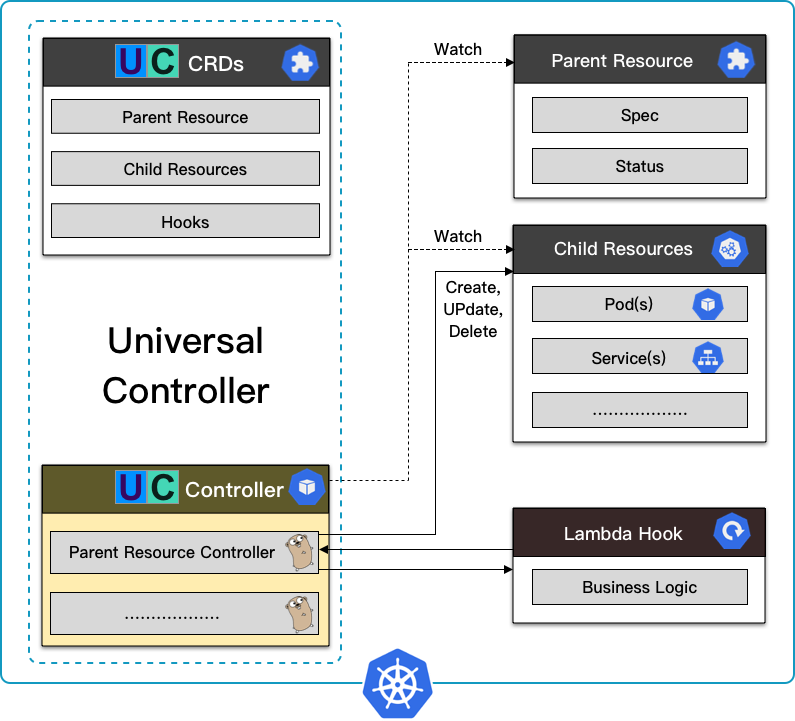
\includegraphics[width= 0.85\textwidth]{pics/uc-arch.png}\\
  \caption{UniversalController架构}\label{fig:uc-arch}
\end{figure}

图\ref{fig:uc-arch}展示了UniversalController的总体架构。UniversalController自身是一个Kubernetes中的controller,负责监视UniversalController CRDs,当有一个新的UniversalController CRD被创建时,它会启动Parent Resource的控制器作为响应。也就是说,UniversalController是控制器的控制器,可以用于管理多个控制器,实现多控制器并存在一个进程中运行。


\section{自定义资源}
\newpage
\begin{lstlisting}[language=yaml,caption=UC CRD,label=listing:1]
apiVersion: apiextensions.k8s.io/v1
kind: CustomResourceDefinition
metadata:
  annotations:
    "api-approved.kubernetes.io": "unapproved, request not yet submitted"
  name: "universalcontrollers.universalcontroller.njuics.cn"
spec:
  group: "universalcontroller.njuics.cn"
  names:
    kind: UniversalController
    listKind: UniversalControllerList
    plural: universalcontrollers
    shortNames:
    - uc
    - uctl
    singular: universalcontroller
  scope: Cluster
...
\end{lstlisting}

YAML代码\ref{listing:1}是UC CRD的定义,通过kubectl向api-server提交这个yaml文件就可以在Kubernetes中注册一种新的资源类型``UniversalController''。这样就成功拓展了Kubernetes APIs,之后就可以使用这个新的API提交资源定义来注册控制器。

\begin{lstlisting}[language=yaml,caption=作为UC CRD示例的catset-controlelr,label=listing:ucsample]
apiVersion: universalcontroller.njuics.cn/v1alpha1
kind: UniversalController
metadata:
  name: catset-controller
spec:
  parentResource:
    apiVersion: mlhub.njuics.cn/v1alpha1
    resource: catsets
  childResources:
    - apiVersion: v1
      resource: pods
      updateStrategy:
        method: RollingRecreate
        statusChecks:
          conditions:
            - type: Ready
              status: "True"
    - apiVersion: v1
      resource: persistentvolumeclaims
  hooks:
    sync:
      webhook:
        url: "http://catset-ctrl.universalcontroller:8080"
\end{lstlisting}

YAML文件\ref{listing:ucsample}是一个UC CRD资源的例子,定义了CatSet资源的控制器,它的行为几乎与Kubernetes原生资源的StatefulSet的控制器一致,是对StatefulSet的二次实现。

一个UC CRD的``spec''有五个字段:parentResource、childResources、resyncPeriodSeconds、generateSelector和hooks。parentResource的类型是ResourceRule,用于指定父资源类型,也就是这个控制器实际管理的资源。ResourceRule只有两个字段``APIVersion''和``Resource'',用于确定一种资源类型。childResources是是一组ResourceRule,用于指定会被控制器生成的子资源类型。resyncPeriodSeconds被用于规定两次调谐之间间隔的时间,设置后就算工作队列当前是空的,但是距离上次调谐过去这么多时间后还是会去调谐。generateSelector是bool型的,如果为真,那么忽略父资源对象的标签选择器(如果存在的话),UniversalController会为其生成独一无二的标签选择器,避免与其他的资源冲突。这里的标签选择器都是为了筛选子资源,符合标签选择器的子资源都会被当做父资源的子资源。hooks是一组定义了控制器行为的lambda hook。

\section{动态类型高级操作接口实现}

Kubernetes的官方Go语言客户端库client-go,提供了dynamic模块,可以用于创建动态客户端,借助于动态客户端,只要知道资源的apiVersion和Kind,就可以对任意一种资源进行操作。UniversalController基于此,实现了支持动态资源类型的informer和indexer,用于订阅特定资源相关事件以及查找特定类型的资源,是自定义控制器的核心组件。

\begin{lstlisting}[language=Go,caption=客户端实现,label=listing:client]
type Clientset struct {
	config    rest.Config
	resources *dynamicdiscovery.ResourceMap
	dc        dynamic.Interface
}
type ResourceClient struct {
	dynamic.ResourceInterface
	*dynamicdiscovery.APIResource
	rootClient dynamic.NamespaceableResourceInterface
}
func New(config *rest.Config, resources *dynamicdiscovery.ResourceMap) (*Clientset, error)
func (cs *Clientset) Resource(apiVersion, resource string) (*ResourceClient, error) {
	// Look up the requested resource in discovery.
	apiResource := cs.resources.Get(apiVersion, resource)
	if apiResource == nil {
		return nil, fmt.Errorf("discovery: can't find resource %s in apiVersion %s", resource, apiVersion)
	}
	return cs.resource(apiResource), nil
}
func (cs *Clientset) resource(apiResource *dynamicdiscovery.APIResource) *ResourceClient {
	client := cs.dc.Resource(apiResource.GroupVersionResource())
	return &ResourceClient{
		ResourceInterface: client,
		APIResource:       apiResource,
		rootClient:        client,
	}
}
func (rc *ResourceClient) AtomicUpdate(orig *unstructured.Unstructured, update func(obj *unstructured.Unstructured) bool) (result *unstructured.Unstructured, err error)

type Unstructured struct {
	// Object is a JSON compatible map with string, float, int, bool, []interface{}, or
	// map[string]interface{}
	// children.
	Object map[string]interface{}
}
\end{lstlisting}

代码段\ref{listing:client}是客户端的结构体和一些方法,UC首先需要用New方法得到一个Clientset类型的对象,对于各种资源,只要知道资源的apiVersion和kind,都可以用这个对象的Resource方法得到一个ResourceClient对象,该对象可以对这类资源进行各类CURD的操作,所有的资源都以Unstructured类型存储,Unstructured中只有一个字典类型的字段,实际是把资源以接近JSON的形式存储起来。

\begin{lstlisting}[language=Go,caption=通知器(Informer)实现,label=listing:informer]
// sharedResourceInformer is the actual, single informer that's shared by
// multiple ResourceInformer instances.
type sharedResourceInformer struct {
	informer cache.SharedIndexInformer
	lister   dynamiclister.Lister
	defaultResyncPeriod time.Duration
	eventHandlers *sharedEventHandler
	close func()
}
func newSharedResourceInformer(client *dynamicclientset.ResourceClient, defaultResyncPeriod time.Duration, close func()) *sharedResourceInformer {
	informer := cache.NewSharedIndexInformer(
		&cache.ListWatch{
			ListFunc: func(opts metav1.ListOptions) (runtime.Object, error) {
				return client.List(opts)
			},
			WatchFunc: client.Watch,
		},
		&unstructured.Unstructured{},
		defaultResyncPeriod,
		cache.Indexers{
			cache.NamespaceIndex: cache.MetaNamespaceIndexFunc,
		},
	)
	sri := &sharedResourceInformer{
		close:               close,
		informer:            informer,
		defaultResyncPeriod: defaultResyncPeriod,
		lister: dynamiclister.New(informer.GetIndexer(), client.GroupVersionResource()),
	}
	sri.eventHandlers = newSharedEventHandler(sri.lister, defaultResyncPeriod)
	informer.AddEventHandler(sri.eventHandlers)
	return sri
}
type ResourceInformer struct {
	sharedResourceInformer *sharedResourceInformer
	informerWrapper        *informerWrapper
}
func newResourceInformer(sri *sharedResourceInformer) *ResourceInformer {
	return &ResourceInformer{
		sharedResourceInformer: sri,
		informerWrapper: &informerWrapper{
			SharedIndexInformer:    sri.informer,
			sharedResourceInformer: sri,
		},
	}
}
\end{lstlisting}

代码段\ref{listing:informer}展示了如何在client的基础之上实现informer,informer会调用client的List和Watch方法来监听资源。SharedInformer的作用是让在一个进程中运行的控制器们共享订阅,避免重复订阅浪费内存和网络带宽。

\section{控制器实现}

图\ref{fig:uc-arch}中的UC Controller和Parent Resource Controller都是自定义控制器。图\ref{fig:client-go-controller-interaction}展现了一个自定义控制器的工作方式。UC Controller和Parent Resource Controller都使用这种经典控制器模式。

UC Controller监视着UC类型的资源,提供了UC相关的服务,同时管理着通过UC CRD创建的自定义控制器。它的``Handle Object''部分确保集群状态与UC CRD期望的一致,也就是保持所有注册的自定义控制器正确运行。

而Parent Resource Controller监视着Parent Resource,它的``Handle Object部分''是UniversalController用户自定义的代码段,一般是若干个函数。

当开发者使用UC的声明式API创建控制器时,开发者需要提供的函数中只包含当前控制器所特有的业务逻辑。这些函数会通过webhook调用,所以开发者可以用任何能够处理网络请求和JSON的编程语言来编写这些函数。

Parent Resource Controller会执行一个调谐循环,在调谐时调用开发者提供的函数,之后再决定做什么。UniversalController为每一个Parent Resource Controller预先准备了调谐循环的通用逻辑,开发者不需要借助代码生成器,可以完全将精力集中在编写调谐函数上。现阶段UniversalController接受的调谐器是Webhook形式的,开发者可以借助serverless工具,例如kubeless或者openFaas,将函数发布成一个Web服务,再提供给控制器。借助UC的API和serverless就可以使开发工作完全集中于业务逻辑,免去了很多琐碎的工作和模版代码。

接下来介绍UC Controller和Parent Resource Controller的``Handle Object''分别是怎么实现的。

\subsection{同步UC CRD资源}
\begin{lstlisting}[language=Go,caption=同步UC CRD,label=listing:syncuniversalcontroller]
func (u *Universalcontroller) syncUniversalController(uc *v1alpha1.
	UniversalController) error {
	if pc, ok := u.parentControllers[uc.Name]; ok {
		if apiequality.Semantic.DeepEqual(uc.Spec, pc.uc.Spec) {
			// Nothing has changed.
			return nil
		}
		pc.Stop()
		delete(u.parentControllers, uc.Name)
	}
	pc, err := newParentController(u.resources, u.dynClient, u.dynInformers, 
		u.mcClient, u.revisionLister, uc, u.numWorkers)
	if err != nil {
		return err
	}
	pc.Start()
	u.parentControllers[uc.Name] = pc
	return nil
}
\end{lstlisting}

代码段\ref{listing:syncuniversalcontroller}中的syncUniversalController方法根据当前的UC CRD资源定义进行调谐,如果这个资源对应的控制器已经存在,并且不需要修改,spec完全一致,那么不用做任何事,本次调谐结束,否则就删除旧的控制器。接下来新建Parent Resource的控制器,并启动,和一般的controller-mananger模式中一样,这个Parent Resource的控制器运行在单独的一个Go协程中,只是此时UC Controller承担了manager的职责,所以UC Controller是controller-controller。

\subsection{同步父资源(Parent Resource)}

代码段\ref{listing:syncparent}展示了Parent Resource Controller对Parent Resource的同步过程:
\begin{enumerate}
	\item claimChildren方法会通过标签选择器找到所有的已经存在的子资源。
	\item 如果Customize Hook非空,通过Customize Hook找到相关资源。
	\item 将Parent Resource、Child Resources、Related Resources放入同步钩子请求体中,调用同步钩子,得到同步结果,其中包含期望的Parent Resource Status和期望的Child Resources,
	\item 先比较已经存在的Child Resources和期望的Child Resources,如果一个资源已经存在,但是与期望不一致,就把它们两个当做JSON对象合并,之后根据更新策略更新得到合并结果;如果一个期望的资源还不存在,就创建它,其实就是执行了``Server-side apply''。
	\item 最后更新Parent Resource Status。
\end{enumerate}

\begin{lstlisting}[language=Go,caption=同步父资源,label=listing:syncparent]
func (pc *parentController) syncParentObject(parent *unstructured.Unstructured) error {
	observedChildren, err := pc.claimChildren(parent)
	if err != nil {
		return err
	}
	relatedObjects, err := pc.customize.GetRelatedObjects(parent)
	if err != nil {
		return err
	}
	syncResult, err := pc.syncRevisions(parent, observedChildren, relatedObjects)
	if err != nil {
		return err
	}
	desiredChildren := common.MakeChildMap(parent, syncResult.Children)
	if syncResult.ResyncAfterSeconds > 0 {
		pc.enqueueParentObjectAfter(parent, time.Duration(syncResult.ResyncAfterSeconds*float64(time.Second)))
	}
	var manageErr error
	if parent.GetDeletionTimestamp() == nil || pc.finalizer.ShouldFinalize(parent) {
		// Reconcile children.
		if err := common.ManageChildren(pc.dynClient, pc.updateStrategy, parent, observedChildren,
			desiredChildren); err != nil {
			manageErr = fmt.Errorf("can't reconcile children for %v %v/%v: %v",
				pc.parentResource.Kind, parent.GetNamespace(), parent.GetName(), err)
		}
	}
	if _, err := pc.updateParentStatus(parent, syncResult.Status); err != nil {
		return fmt.Errorf("can't update status for %v %v/%v: %v", pc.parentResource.Kind,
			parent.GetNamespace(), parent.GetName(), err)
	}
	return manageErr
}
\end{lstlisting}


\section{声明式的更新策略}
\subsection{更新策略介绍}
UniversalController提供了很多更新策略,开发者可以通过声明式接口使用它们,而不用写任何代码。
\begin{itemize}
	\item 待删除后更新(OnDelete):不更新现有的子资源,直到它被其他的客户端例如kubectl删除。
	\item 立刻重建(ReCreate):立即删除任何不符合期望状态(state)的子资源,并根据期望状态(state)重新创建。
	\item 就地更新(InPlace):立刻就地更新任何不符合期望状态(state)的子资源。
	\item 滚动重建(RollingRecreate):每次调谐删除一个与期望状态(state)不同的子资源,并在处理下一个子资源之前根据期望状态(state)重建它。在任意时刻,如果已经更新的子资源中有一个或多个状态检查失败,则暂停滚动更新。
	\item 滚动就地更新(RollingInPlace):每次更新一个与期望状态(state)不同的子资源。如果已经更新的子资源中有一个或多个状态检查失败,则暂停滚动更新。
\end{itemize}

不同的资源适合不同的更新策略,例如Pod一般会用ReCreate或者RollingRecreate,因为当一个已经在Kubernetes中存在的Pod,它能修改的只有metadata中的标签(labels)和附加说明(annotations),spec中的字段都不能修改,如果需要修改,就只能删除重建。而Deployment除了名字和命名空间都可以修改,用InPlace或者RollingInPlace显然更合适。

\subsection{滚动更新版本控制}\label{section:rolling-control}
ControllerRevision是UniversalController使用的一个内部API,用于实现声明式的滚动更新,主要受到Kubernetes原生资源StatefulSet和DaemonSet使用的ControllerRevision启发后实现。

每个ControllerRevision都与一个资源相关,名称是该资源的类型、资源所在的apiGroup以及版本后缀组成的。版本后缀是对该资源指定字段的哈希结果。

默认情况下,一旦一个特定的父资源被删除,属于该资源的ControllerRevision们会被垃圾回收处理掉。但是,也可以在父资源的删除过程中抛弃ControllerRevision,不再与这个父资源有关系的ControllerRevision也就不会被删除了,就可以创建另一个父资源来接管它。接管的规则基于父资源的标签选择器,和ReplicaSet接管Pods的方式一样。

\begin{lstlisting}[language=yaml,caption=ControllerRevision示例,label=listing:controllerrevision]
apiVersion: universalcontroller.njuics.cn/v1alpha1
kind: ControllerRevision
metadata:
  name: catsets.universalcontroller.njuics.cn-5463ba99b804a121d35d14a5ab74546d1e8ba953
  labels:
    app: nginx
    component: backend
    universalcontroller.njuics.cn/apiGroup: universalcontroller.njuics.cn
    universalcontroller.njuics.cn/resource: catsets
parentPatch:
  spec:
    template:
      [...]
children:
- apiGroup: ""
  kind: Pod
  names:
  - nginx-backend-0
  - nginx-backend-1
  - nginx-backend-2
\end{lstlisting}

YAML文件\ref{listing:controllerrevision}是ControllerRevision的一个例子,parentPatch字段存储了父资源的部分表示,它只包含UC CRD的revisionHistory字段列出的那些参与滚动更新的字段,默认是spec。

例如,如果一个UC CRD的revisionHistory是数组[\"spec.template\"],那么parentPath只会包含spec.template和嵌套在其中的子字段。

这样就可以在滚动更新的过程中做出选择性行为。任何不属于revisionHistory的字段如果被更新,更新都会立即生效,而不是进行滚动更新。

children字段存储了一个``属于''这个ControllerRevison的子资源列表,UniversalController就是通过这个字段跟踪一个子资源属于哪个ControllerRevision。在滚动更新过程中,如果一个还没有更新的Pod被用户通过kubectl删除了,那么它应该重建它被删除之前的版本,而不是最新版本,以保证滚动更新的粒度与次序不被打乱。

当UniversalController决定将一个子资源更新到另一个版本时。它首先会更新相关的ControllerRevison来表达这个意图,这些更新被提交后,它就会根据所配置的子资源更新策略开始更新该子资源。这确保了滚动更新的中间结果在api-server中被持久化,就算UniversalController重启,也能从中断的位置继续更新。

children字段的值是按照apiGroup和kind进行分组的。对于每个apiGroup和kind的组合,存储了一个对象名称列表。
\section{调谐器接口实现}
在示例的YAML文件\ref{listing:ucsample}中hooks.sync就定义了当前控制器使用的调谐器。编写调谐器是在开发者基于UniversalController开发Operator时唯一需要的自定义代码编写工作。编写完成后需要以webhook的形式发布出来,借助serverless工具即可省去网络相关代码的编写。之后再UC CRD的相应字段填写服务地址就完成了控制器的配置。UC CRD中的Webhook结构如表\ref{table:webhook}所示。在webhook中,service的结构如表\ref{table:service-reference}所示。

\begin{table}
  \centering
  \begin{tabular}{ccp{50mm}}
    \toprule
    \textbf{字段} & \textbf{Go类型} & \textbf{说明} \\
    \midrule
    url  & string  & 完整的url地址,优先级比path和service的组合高\\
    timeout  & Duration   &  时限,过期未收到回复就是请求超时 \\
    path     & string  &  请求链接的后缀 \\
    service    & ServiceReference   &  应该被发送请求的K8s Service \\
    \bottomrule
  \end{tabular}
  \caption{Webhook}\label{table:webhook}
\end{table}

\begin{table}
  \centering
  \begin{tabular}{ccp{50mm}}
    \toprule
    \textbf{字段} & \textbf{Go类型} & \textbf{说明} \\
    \midrule
    name  & string  & 该Service的名称\\
    namespace  & string   &  该Service的命名空间 \\
    port     & int32  & 该Service提供服务的接口 \\
    protocol    & string   &  协议,默认为http \\
    \bottomrule
  \end{tabular}
  \caption{Service Reference}\label{table:service-reference}
\end{table}

\paragraph{Hooks}
在UC CRD的spec中,hooks字段有以下三个子字段:sync、finalize和customize。sync用于指定如何调用同步钩子。finalize用于指定如何调用收尾(finalize)钩子。customize用于指定如何调用Customize钩子。它们都对应了一种Hook类型,下面开始分别介绍。

\subparagraph{同步钩子}

同步钩子被用来指定为给定的父资源创建或维护那些子资源,即期望状态(state)。根据UC CRD的spec,UniversalController会收集所有需要的资源,并向同步钩子发送最新观察到的状态(state)。同步钩子返回期望状态后,UniversalController会开始通过一系列操作向它收敛,操作包括适当地创建、删除和更新对象。

可以简单的把同步钩子看做一个脚本,它生成json发送到``server-side apply'',同时,与一次性的客户端生成器不同的是,这个脚本可以观察到集群中最新的状态(state),并且会在观察到的状态(state)发生变化时自动被执行。

\textbf{同步钩子请求}

一个请求中只会包含一个父资源,所以同步钩子一次只需要考虑一个父资源。

请求体是一个JSON对象,它的字段包括parent、children、related和finalizing。parent对象是一个json形式的父资源,和用kubectl get <parent-resource> <parent-name> -o json得到的结果一样。children对象存储了与父资源相关的子资源们,是通过标签选择器筛选得到的。related对象只有当Customize钩子存在时,会存储相关资源,否则为空。finalizing是布尔型的,在调用同步钩子是始终为false。

children对象的每个字段都代表UC CRD的spec中指定的子资源类型之一。每个子资源类型的字段名是<kind>.<apiVersion>。举例来说,Pods的字段名是Pod.v1,而StatefulSets的字段名是StatefulSet.apps/v1。

在每个字段中(例如在children['Pod.v1']中),存储这一个字典,键是当前资源标识,值是该资源的json表示。如果父资源和子资源的作用域相同,都是集群的或者都是命名空间的,那么键就只是子资源的名称,如果父资源是集群作用域,而子资源是命名空间作用域,那么键的形式是{.metadata.namespace}/{.metadata.name}。这是为了区分可能存在的在不同命名空间的两个同名子资源。父资源是命名空间作用域而子资源是集群作用域的情况不可能出现。举例来说,如果父资源在my-namespace命名空间下,那么在my-namespace命名空间下的一个名称为my-pod的Pod会被存储在request.children['Pod.v1']['my-pod']。如果父资源是集群作用域的,这个Pod会被存储在request.children['Pod.v1']['my-namespace/my-pod']。每个子资源类型总是有一个入口,即使在同步时没有观察到该类型的子资源。例如,如果Pod是子资源类型之一,但没有任何现有的Pods资源与父资源的选择器相匹配,请求体的形式是:
\begin{lstlisting}[language=json,caption=请求体,label=listing:7]
{
  "children": {
    "Pod.v1": {}
  }
}
\end{lstlisting}
而不是
\begin{lstlisting}[language=json,caption=异常请求体,label=listing:8]
{
  "children": {}
}
\end{lstlisting}

related字段下存储着相关资源对象,格式与children字段下的对象相同,表示与给定父资源的Customize钩子响应相匹配的资源,这些资源不由控制器管理,因此不可修改,但可以将它们当做系统上下文,进而得到子资源的期望配置。当观察到相关资源被更新时,就算父资源和子资源都没有变化,同步钩子也会被触发。

\textbf{同步钩子响应}

同步钩子的响应体的字段包括status、children和resyncAfterSeconds。status是一个JSON对象,将完全取代父资源中的状态字段。children是一组JSON对象组成的列表,代表所有期望存在的子资源。resyncAfterSeconds是下次同步的时间间隔,以秒为单位,类型是浮点数。

状态(status)的设置完全由用户代码段决定,状态(status)应该根据最后观察到的状态(state)来填写,是一个当前值,而不是期望值。

响应体中的children字段是一个对象数组,而不是请求体中那样的字典,每一个对象都是一个期望存在的子资源。UniversalController按照类型和名称对发送的对象进行分组,以方便用户简化脚本,但实际上这是多余的,因为每个对象都包含自己的apiVersion、kind和metadata.name。

任何在请求体中存在的子资源,如果调谐逻辑拒绝在响应体中返回,它会被UniversalController在收到响应后删除。但是,调谐逻辑不应该直接把请求中的子资源复制到返回结果中,因为它们的形式不同,返回的结果应该完全根据父资源的specification和系统上下文重新生成。用户应该把响应体中的每个子资源看作是被发送到``kubectl apply'',只需要设置用户关心的字段。

如果返回的resyncAfterSeconds被设置为一个大于0的值,同步钩子在延迟一段时间后会被再次调用,请求体中的parent字段的值依然是这个特定的父资源,其他字段依据父资源设置。这个设置时一次性的,不会周期性重新同步,而且只针对这个特定的父资源。

\subparagraph{Finalize钩子}
如果定义了finalize钩子,UniversalController将为父资源添加一个finalizer,这将防止它被直接删除,直到finilize钩子执行完,并且钩子的响应表明清理已经完成,它才能真正的被删除。

这对于清理可能在外部系统中创建的资源是很有用的。如果定义finalize钩子,那么当一个父对象被删除时,垃圾回收器会立即删除所有的子对象,而不会调用任何钩子。

finalize钩子的语义大多与同步钩子的语义相当。UniversalController将尝试调谐在children字段中返回的期望状态(state),并将在父资源上设置状态(status)。主要的区别是,当父资源正在被删除且需要清理时,会调用finalize钩子而不是同步钩子。

当观察到的状态发生变化时,UniversalController可能会多次调用finalize钩子,甚至可能是在一次表明已经完成finalize的调用之后。用户编写的处理程序应该知道如何检查还需要做什么,如果没有什么需要做的,就报告成功。

同步钩子和finalize钩子都有一个叫做finalizing的请求字段,用来指示到底调用了哪个钩子,在同步钩子请求中始终为false,在finalize钩子请求中始终为true。这让用户可以自己选择将 finalize钩子作为一个单独的处理程序还是作为同步处理程序中的一个分支来实现,这取决于它们共享多少逻辑。要为两者使用相同的处理程序,只需定义一个 finalize 钩子,并将其设置为与同步钩子相同的值。

\textbf{finalize钩子请求}

finalize钩子的请求体格式与同步钩子的完全相同,只是finalizing字段始终为true而已。如果同步钩子和finalize钩子共享同一段处理程序,可以使用finalizing字段来判断是该清理还是进行正常的同步。如果为finalize定义了一个单独的处理程序,就不需要检查finalizing字段,因为它总是为真。

\textbf{finalize钩子响应}

finalize钩子响应体拥有所有同步钩子响应体的字段,但还有一个额外的字段finalized,是一个布尔值,用于表示清理是否已经结束。

\subparagraph{Customize钩子}

如果定义了Customize钩子,UniversalController会询问它哪些资源是相关资源,应该放入同步钩子和finalize钩子的请求中。这在有些场景下非常有用。一个例子是,用户想实现一个控制器将指定的ConfigMaps复制到每个Namespace中。另一个例子是有些控制器希望能够引用相关对象的一些信息,例如,从有些Pod资源获取env部分。如果没有定义Customize钩子,那么同步钩子和finalize钩子的请求体中related都将是空的。

当前Customize钩子的请求体中不会提供任何关于集群当前状态(state)的信息,只包含父资源,所以相关对象的集合只取决于父资源的spec。

\textbf{Customize钩子请求}

Customize钩子的请求体只有一个parent字段,用于存储一个父资源的json表示。

\textbf{Customize钩子响应}

Customize钩子的响应体只有一个字段``relatedResources'',存放了一组JSON对象,每个JSON对象是一个ResourceRule,用于筛选资源。

ResourceRule的字段包括apiVersion、resource、labelSelector、namespace和name。apiVersion是资源的apiVersion,例如apps/v1、v1、batch/v1等。resource是资源的小写名称,例如deployments, replicasets, statefulsets。labelSelector是用于筛选资源的标签选择器,如果为空,用namespace和names字段去定位资源。namespace是选填项,指资源所在的命名空间。name也是选填项,代表资源名称列表。

如果设置了labelSelector,namspace字段和name字段就应该都为空,反之亦然,它们不应该被同时设置,它们代表了两种不同的资源筛选方式,在一次筛选中只能使用一种。

UniversalController收到Customize钩子响应后就回去用这一系列资源筛选规则找到符合调节的资源们,并放入同步或finalize钩子的请求体中。

\section{小结}
本章详细介绍了各个组件或功能在UniversalController中是设计与实现的,涉及到了各方面的细节。

%%%%%%%%%%%%%%%%%%%%%%%%%%%%%%%%%%%%%%%%%%%%%%%%%%%%%%%%%%%%%%%%%%%%%%%%%%%%%%%
\chapter{实验评估}\label{chapter_experiments}
\section{用例1:重新实现sample-controller}\label{section:sample-controller}
\subsection{介绍}
sample-controller是Kubernetes官方提供的一个Operator编写样例,项目地址是https://github.com/kubernetes/sample-controller。

它是一个简单的控制器,监视通过CustomResourceDefinition定义的Foo资源,为每个Foo保证一个对应的Deployment存在。sample-controller展示了一个标准的Operator是如何实现并工作的,使用client-go与Kubernetes api-server交互,编写控制器的各个组件,没有使用更高级的抽象包。
\subsection{实现}

\begin{lstlisting}[language=yaml,caption=sample-controller的配置文件,label=listing:sample-controller-config]
apiVersion: universalcontroller.njuics.cn/v1alpha1
kind: UniversalController
metadata:
  name: sample-controller
spec:
  generateSelector: true
  parentResource:
    apiVersion: njuics.cn/v1alpha1
    resource: foos
  childResources:
  - apiVersion: apps/v1
    resource: deployments
    updateStrategy:
      method: InPlace
  hooks:
    sync:
      webhook:
        url: "http://sample-controller.universalcontroller:8080"
\end{lstlisting}

YAML文件\ref{listing:sample-controller-config}是sample-controller的定义文件,7-9行指定了它需要处理的父资源类型,10-12行指定了子资源类型。18行是用户的调谐逻辑的入口。


\begin{lstlisting}[language=JavaScript,caption=sample-controller的实现代码,label=listing:sample-controller]
module.exports =  {
  handler: (event, context) => {
    let observed = event['data'];
    return reconcile(observed.parent, observed.children);
  }
};
var reconcile = function (foo, children) {
    let desiredChildren = [];
    let currentStatus = {};
    let allDeploys = children['Deployment.apps/v1'];
    let fooDeploy = allDeploys ? allDeploys[foo.spec.deploymentName] : null;
    let replicas = fooDeploy ? fooDeploy.status.availableReplicas : 0;
    currentStatus = {availableReplicas: replicas};// Set the status of Foo
    desiredChildren = [desiredDeployment(foo)];
    return {status: currentStatus, children: desiredChildren};
}
var desiredDeployment = function (foo) {
  let lbls = {app: "sample"};
  let deploy = {
    apiVersion: "apps/v1",
    kind: "Deployment",
    metadata: {
      name: foo.spec.deploymentName,
      namespace: foo.metadata.namespace,
    },
    spec: {
      replicas: foo.spec.replicas,
      selector: {matchLabels: lbls},
      template: {
        metadata: {labels: lbls},
        spec: {
          containers: [{
              name: "nginx",
              image: "nginx:stable"
            }]
        }
      }
    }
  };
  return deploy;
};
\end{lstlisting}

JavaScript代码\ref{listing:sample-controller}就是所有需要写的代码,而不是一个代码段。它的逻辑很简单,从请求体中取出Foo资源,根据它的定义生成期望的Deployment,Foo资源的status只有一个字段表示可用的副本数,如果Deployment还不存在,可用副本数为0,否则就是该Deployment的status.availableReplicas的值,最后将status和Deployment返回即可。

接下来借助kubeless将这个函数部署成web服务,只需要一条命令:
kubeless -n universalcontroller function deploy sample-controller --runtime nodejs10 --from-file sync.js --handler sync.handler

之后在universalcontroller命名空间下会生成一个名叫sample-controller的Service资源和一个名叫sample-controller的Deployment资源,于是在集群内部就可以用http://sample-controller.universalcontroller:8080访问这个服务,这个url就是要生成的controller使用的同步钩子。最后使用``kubectl apply''命令提交YAML文件\ref{listing:sample-controller-config}完成控制器的注册。
\section{用例2:重新实现tf-operaotr}
\subsection{介绍}
tf-operator由kubeflow社区开发,项目地址为https://github.com/kubeflow/tf-operator,它提供了TFJob这个Kubernetes自定义资源,使其能够轻松地在Kubernetes上运行分布式或非分布式TensorFlow任务。
\subsection{实现}

\begin{lstlisting}[language=yaml,caption=tensorflowjob-controller的配置文件,label=listing:tensorflow-controller-config]
apiVersion: universalcontroller.njuics.cn/v1alpha1
kind: UniversalController
metadata:
  name: tensorflowjob-controller
spec:
  parentResource:
    apiVersion: mlhub.njuics.cn/v1alpha1
    resource: tensorflowjobs
  childResources:
    - apiVersion: v1
      resource: services
      updateStrategy:
        method: InPlace
    - apiVersion: v1
      resource: pods
      updateStrategy:
        method: ReCreate
  hooks:
    sync:
      webhook:
        url: "http://tensorflow-controller.universalcontroller:8080"
\end{lstlisting}

YAML文件\ref{listing:tensorflow-controller-config}是tensorflowjob-controller的声明式定义。

\begin{lstlisting}[language=JavaScript,caption=tensorflowjob-controller的实现代码,label=listing:tensorflowjob-controller]
let tfjob = observed.parent;
let status = deepCopy(tfjob.status);
let observedPods = Object.values(observed.children['Pod.v1']);
let replicas = tfjob.spec.tfReplicaSpecs;
for (let rtype of Object.keys(replicas)) {
  let spec = replicas[rtype];
  let rt = rtype.toLowerCase();
  status.replicaStatuses[rtype] = {active: 0, succeeded: 0, failed: 0};
  let pods = filterPodsForReplicaType(observedPods, rt);
  let numReplicas = spec.replicas;
  let podSlices = getPodSlices(pods, numReplicas);
  for (let index = 0; index < podSlices.length; index++) {
    if (index < numReplicas) {
      desiredChildren.push(newSVC(tfjob, rtype, index));
    }
    let podSlice = podSlices[index];
    if (podSlice.length === 1) {
      let pod = podSLice[0];
      let exitCode = getContainerExitCode(pod);
      if (spec.restartPolicy === 'ExitCode') {
        if (pod.status.phase === 'Failed' && isRetryableExitCode(exitCode)) {
          updateJobConditions(status, 'Restarting', 'TFJobRestarting',
              `TFJob ${tfjob.metadata.name} is restarting because ${rtype} replica(s) failed.`);
          continue;
        }
      }
      if (pod.status.phase === 'Running') {
        status.replicaStatuses[rtype].active++;
      } else if (pod.status.phase === 'Succeeded') {
        status.replicaStatuses[rtype].succeeded++;
      } else if (pod.status.phase === 'Failed') {
        status.replicaStatuses[rtype].failed++;
      }
    }
    if (index < numReplicas) {
      let masterRole = isMasterRole(replicas, rtype, index);
      desiredChildren.push(newPod(tfjob, rt, index, spec, masterRole, replicas));
    }
  }
}
\end{lstlisting}

tf-operator依然用JavaScript实现,但实现逻辑相当复杂,总代码行数为408行,核心代码为代码段\ref{listing:tensorflowjob-controller}。原版tf-operator中的逻辑都转译了过来,包括根据不同的副本类型使用当前tfjob资源中相应的模版来创建Pod,为每一个Pod创建一个Service,分别统计每种副本的状态来更新tfjob的status等。

接下来借助kubeless将这个函数部署成web服务,部署命令为:

kubeless -n universalcontroller function deploy tensorflow-controller --runtime nodejs10 --from-file sync1.js --handler sync1.handler

之后在universalcontroller命名空间下会生成一个名叫tensorflow-controller的Service资源和一个名叫tensorflow-controller的Deployment资源,于是在集群内部就可以用http://tensorflow-controller.universalcontroller:8080访问这个服务,这个url就是要生成的controller使用的同步钩子。

\section{用例3:CatSet与滚动更新}\label{section:catset}
\subsection{介绍}
CatSet是对Kubernetes原生资源StatefulSet的重新实现,同时可以展示滚动更新的使用。
\subsection{实现}

\begin{lstlisting}[language=yaml,caption=catset-controller的配置文件,label=listing:catset-controller-config]
---
apiVersion: universalcontroller.njuics.cn/v1alpha1
kind: UniversalController
metadata:
  name: catset-controller
spec:
  parentResource:
    apiVersion: mlhub.njuics.cn/v1alpha1
    resource: catsets
    revisionHistory:
      fieldPaths:
        - spec.template
  childResources:
    - apiVersion: v1
      resource: pods
      updateStrategy:
        method: RollingRecreate
        statusChecks:
          conditions:
            - type: Ready
              status: "True"
    - apiVersion: v1
      resource: persistentvolumeclaims
  hooks:
    sync:
      webhook:
        url: "http://catset-controller.universalcontroller:8080"
    finalize:
      webhook:
        url: "http://catset-controller.universalcontroller:8080"
\end{lstlisting}

\begin{lstlisting}[language=yaml,caption=CatSet资源示例,label=listing:catset-sample]
apiVersion: mlhub.njuics.cn/v1alpha1
kind: CatSet
metadata:
  name: nginx-backend
spec:
  serviceName: nginx-backend
  replicas: 3
  selector:
    matchLabels:
      app: nginx
  template:
    metadata:
      labels:
        app: nginx
        component: backend
    spec:
      terminationGracePeriodSeconds: 1
      containers:
      - name: nginx
        image: gcr.io/google_containers/nginx-slim:0.8
        ports:
        - containerPort: 80
          name: web
        volumeMounts:
        - name: www
          mountPath: /usr/share/nginx/html
  volumeClaimTemplates:
  - metadata:
      name: www
      labels:
        app: nginx
        component: backend
    spec:
      accessModes: [ "ReadWriteOnce" ]
      resources:
        requests:
          storage: 1Gi
\end{lstlisting}

YAML文件\ref{listing:catset-controller-config}是catset-controller的声明式定义。YAML文件\ref{listing:catset-sample}是一个CatSet资源的示例,CatSet的spec结构与StatefulSet的spec结构完全一样。

\begin{lstlisting}[language=JavaScript,caption=生成Pod和PVC,label=listing:catset]
module.exports = {
  handler: (event, context) => {
    let observed = event.data;
    let desiredChildren = [];
    let currentStatus = {};
    let finalized = false;
    let catset = observed.parent;
    // Arrange observed Pods by ordinal.
    let observedPods = {};
    if (observed.children && observed.children['Pod.v1']) {
      for (let pod of Object.values(observed.children['Pod.v1'])) {
        let ordinal = getOrdinal(catset.metadata.name, pod.metadata.name);
        if (ordinal >= 0) observedPods[ordinal] = pod;
      }
    }
    if (observed.finalizing) {
      // If the parent is being deleted, scale down to zero replicas.
      catset.spec.replicas = 0;
      // Mark the finalizer as done if there are no more Pods.
      finalized = (Object.keys(observedPods).length === 0);
    }
    for (var ready = 0; ready < catset.spec.replicas && isRunningAndReady(observedPods[ready]); ready++) ;
    currentStatus = {replicas: Object.keys(observedPods).length, readyReplicas: ready};
    let desiredPods = {};
    for (let ordinal in observedPods) {
      desiredPods[ordinal] = newPod(catset, ordinal);
    }
    // Fill in one missing Pod if all lower ordinals are Ready.
    if (ready < catset.spec.replicas && !(ready in desiredPods)) {
      desiredPods[ready] = newPod(catset, ready);
    }
    // If all desired Pods are Ready, see if we need to scale down.
    if (ready === catset.spec.replicas) {
      let maxOrdinal = Math.max(...Object.keys(desiredPods));
      if (maxOrdinal >= catset.spec.replicas) {
        delete desiredPods[maxOrdinal];
      }
    }
    // List Pods in descending order, since that determines rolling update order.
    for (let ordinal of Object.keys(desiredPods).sort((a, b) => a - b).reverse()) {
      desiredChildren.push(desiredPods[ordinal]);
    }
    if (catset.spec.volumeClaimTemplates) {
      let desiredPVCs = {};
      for (let template of catset.spec.volumeClaimTemplates) {
        let baseName = `${template.metadata.name}-${catset.metadata.name}`;
        for (let i = 0; i < catset.spec.replicas; i++) {
          desiredPVCs[i] = newPVC(`${baseName}-${i}`, template);
        }
        // Also generate a desired state for existing PVCs outside the range.
        // PVCs are retained after scale down, but are deleted with the CatSet.
        if (observed.children && observed.children['PersistentVolumeClaim.v1']) {
          for (let pvc of Object.values(observed.children['PersistentVolumeClaim.v1'])) {
            if (pvc.metadata.name.startsWith(baseName)) {
              let ordinal = getOrdinal(baseName, pvc.metadata.name);
              if (ordinal >= catset.spec.replicas) desiredPVCs[ordinal] = newPVC(pvc.metadata.name, template);
            }
          }
        }
      }
      desiredChildren.push(. ..Object.values(desiredPVCs));
    }
    return {children:desciredChildren, status:currentStatus,finalized:finalized};
  },
};
\end{lstlisting}

CatSet的控制器依然用JavaScript实现,代码段\ref{listing:catset}是主逻辑,需要生成带编号的Pods和PVC(如果有的话),为了支持滚动更新,还要把Pods按照编号排好序再返回,因为滚动更新是按照调谐结果中子资源列表中的顺序逐个更新的。


%\section{用例4:Customize钩子的用法}
%\subsection{介绍}
%本文实现了globalconfigmap-operator,用于介绍Customize钩子的用法。
%\subsection{实现}
%
%\begin{lstlisting}[language=Python,caption=,label=listing:]
%
%\end{lstlisting}
%
%\begin{lstlisting}[language=yaml,caption=globalconfigmap-controller的配置,label=listing:globalconfigmap-controller-config]
%apiVersion: universalcontroller.njuics.cn/v1alpha1
%kind: UniversalController
%metadata:
%  name: globalconfigmap-controller
%spec:
%  generateSelector: true
%  parentResource:
%    apiVersion: mlhub.njuics.cn/v1alpha1
%    resource: globalconfigmaps
%  childResources:
%  - apiVersion: v1
%    resource: configmaps
%    updateStrategy:
%      method: InPlace
%  hooks:
%    sync:
%      webhook:
%        url: http://globalconfigmap-controller.universalcontroller/sync
%    customize:
%      webhook:
%        url: http://globalconfigmap-controller.universalcontroller/customize
%\end{lstlisting}
%
%yaml文件\ref{globalconfigmap-controller-config}是用于在UniversalController中注册一个控制器的配置文件。
%
%\subsection{总结}
%因为globalcomfigmap-operator需要把一个ConfigMap复制到每个命名空间,所以用户编写同步钩子时需要知道集群当前有哪些命名空间。

\section{用例对比与分析}

\begin{figure}[htbp]
  \centering
  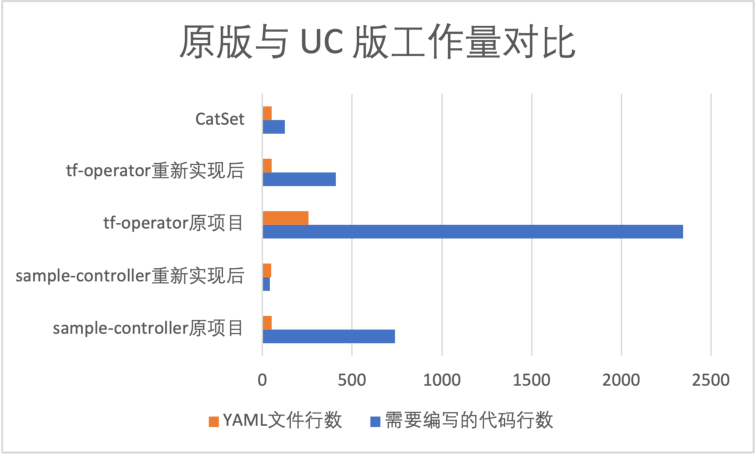
\includegraphics[width=0.75\textwidth]{pics/operator-line.pdf}\\
  \caption{原版与UC版代码行数比较}\label{fig:operator-cl}
\end{figure}

图\ref{fig:operator-cl}直观地展示了直接用client-go实现Operator与借助UC实现在工作量上的巨大差距。

原来的sample-controller是用Go语言实现的,总代码行数为1701,剔除使用代码生成工具生成的代码后代码行数为739。而借助UniversalController,可以用JavaScript来编写业务逻辑,并且controller配置和代码加起来也只有58行。对于功能简单的Operator,借助UniversalController可以实现代码量很少的极速开发。

原版tf-operator主要使用了client-go包,实现了一个标准的Operator,Go代码行数为17155,剔除使用代码生成工具生成的代码以及测试代码后代码行数为2344。在UniversalController之上实现的版本只需要四百多行JavaScript代码就能实现同样的功能。这个用例主要是为了展示UniversalController具备在实现复杂Operator时依然保持工作量相对较小的能力。

CatSet重新实现了StatefulSet,并且支持滚动更新。为了支持滚动更新,开发者只需要编写YAML文件\ref{listing:catset-controller-config}的第16到第21行,为pods子资源加上滚动更新策略,以及编写代码\ref{listing:catset}的第38行到第40行将期望存在的Pods按照序号降序排列即可。开发者总共只添加了9行代码就让CatSet支持了滚动更新,而为了让StatefulSet支持滚动更新,Kubernetes开发者改动了业务逻辑、模版文件、生成的代码,总共涉及到了超过9000行的改动\cite{statefulsetupdate}。UC提供的声明式接口帮助开发者快速地使自己的应用支持滚动更新。

\section{性能测试}

Operator一般都不是计算型任务,运行时CPU的占用率极低,特别是在(超)小型集群中,接近于0。但是因为要监视资源,也就是订阅并且建立缓存,内存开销和网络开销呈线性增长。所以性能测试主要从这两个维度进行分析。

\subsection{实验环境}

在表\ref{table:test-env}所描述的集群上搭建了Kubernetes集群用于实验。
\begin{table}
  \centering
  \begin{tabular}{cp{60mm}c}
    \toprule
    \textbf{硬件类型} & \textbf{型号} & \textbf{规格} \\
    \midrule
    CPU  & Intel(R) Xeon(R) CPU E5-2630 v4 @ 2.20GHz  & 20核\\
    GPU  & NVIDIA 1080Ti   &  2 \\
    内存     & DDR4 & 128GB \\
    网卡    & Mellanox Technologies MT26448   & 10Gbps \\
    磁盘 & TOSHIBA MG04SCA20EN & 2TB \\
    \bottomrule
  \end{tabular}
  \caption{四节点集群的服务器配置}\label{table:test-env}
\end{table}

\subsection{对比方法}

我设计了八种场景,用于论证相比于部署多个Operators,使用UniversalController可以消耗更少的内存和网络带宽。每个场景准备前都要清理环境,重新安装Kubernetes,之后部署100个只执行``sleep 365d''的Pod当做负载。我还实现了一种donothing-operator,它的CRD为DoNothing-<随机后缀>,它的控制器会订阅Pod和PVC,但是什么都不干。实现它的目的是为了方便实验。

接下来每个场景会安装不同的Operators:
\begin{itemize}
	\item \textbf{场景1}:不安装任何Operator。
	\item \textbf{场景2}:只安装UniversalController。
	\item \textbf{场景3}:只安装原版的tf-operator。
	\item \textbf{场景4}:先安装UniversalController,再安装重新实现的tf-operator。
	\item \textbf{场景5}:安装donothing-operator和原版的tf-operator。
	\item \textbf{场景6}:先安装UniversalController,再安装重新实现的tf-operator以及catset-operator。
	\item \textbf{场景7}:安装两个donothing-operator和原版的tf-operator。
	\item \textbf{场景8}:先安装UniversalController,再安装重新实现的tf-operator以及catset-operator,最后安装用UC重新实现的donothing-operator。
\end{itemize}

一个Opeator在安装之后,首先会与kube-apiserver进行同步,建立它关心的资源的缓冲,所有启动之后会有一小段网络流量高峰,之后回落,再趋于平稳,内存也是先快速增长,之后趋于平稳。我会将每个场景中api-server在Operators启动后的前5分钟内上传的总数据量作为网络负载参考量,将之后5分钟内Operators所占用的总内存的平均值作为内存负载参考量。

\subsection{实验结果}
表\ref{table:test}汇总了各个场景的结果。场景1中没有任何Operator,但是每个节点的Kubelet都需要与api-server同步信息,所有也有很多数据需要传输。场景2中安装了UniversalController,但是UC它只会监听UC CRD,集群中没有任何UC CRD,所以api-server的网络负载几乎不变。场景3中tf-operator需要订阅TFJob、Pod、Service,所以api-server的网络负载增加了不少。

对比场景3和场景4可以看到,因为UC Controller自身带来的负载,重新实现的tf-operator的内存和网络负载都要比原版的tf-operator要高。

但是对比场景5和场景6可以看到,再增加一个operator后,场景5的内存和网络负载要更高,比场景3增长很多,而场景6与场景4的负载很接近。tf-operator和catset-operator都需要订阅Pod资源,但是当它们都部署在UniversalController之上时,Pod资源只会被订阅一次,这部分就不会带来额外的负载,catset-operator还需要订阅Service和CatSet,但是我们当前集群中主要的资源都是Pod,Service很少,还没有CatSet,所以也没有产生很多负载。场景8相对场景6的资源增量,以及场景7相对场景5的资源增量也反映了这一点。

借助UniversalController的共享信息器(SharedInformer),当部署多个Operators时,部署在UniversalController之上要比每个单独部署占用更少的内存和网络带宽。
\begin{table}
  \centering
  \begin{tabular}{ccc}
    \toprule
    \textbf{场景编号} & \textbf{Operators内存总用量(MB)} & \textbf{5分钟内上传数据量(KB)} \\
    \midrule
    1  & 0 & 11995.14 \\
    2  & 12.52  &  12012.05 \\
    3  & 13.87  & 13297.24 \\
    4  & 19.18 &  13438.46 \\
    5  & 25.78  & 14529.64 \\
    6  & 21.93  & 13542.36 \\
    7  & 37.84  & 15839.75 \\
    8  & 23.13  & 13708.53 \\
    \bottomrule
  \end{tabular}
  \caption{性能测试}\label{table:test}
\end{table}

\section{小结}
本章设计了多个用例,用UniversalController实现了三个功能各异的Kubernetes Operators,验证了UniversalController可以简化Operator的实现,并且有很强的通用性。

本章设计的性能测试也证实UniversalController借助于共享通知者(sharedInformer),避免了重复订阅同一个资源,相比于一般的多控制器部署方式对内存和网络的占用更小。
%%%%%%%%%%%%%%%%%%%%%%%%%%%%%%%%%%%%%%%%%%%%%%%%%%%%%%%%%%%%%%%%%%%%%%%%%%%%%%%
% 学位论文的正文应以《结论》作为最后一章
\chapter{总结和展望}\label{chapter_concludes}
\section{工作总结}
随着云计算的蓬勃发展,新技术不断涌现。Docker和Kubernetes的出现更是重要的里程碑。Kubernetes已经成为了容器编排的实时标准,是云计算重要的基础设施。但是Kubernetes提供的现有APIs不一定能够很好的满足使用者的需求,使用者经常需要去扩展Kubernetes以更好的支持自己的应用的部署、更新和维护。最主流的Kubernetes扩展方式就是Kubernetes Operators,大量的Operators开始在开源社区出现。然而,编写一个Operator并不容易,具有相当高的门槛,并且需要付出大量的精力和时间。Operator开发人员需要一定程度的Kubernetes和分布式系统知识,需要写大量的模版代码或者使用代码生成工具,编写出的Operator帮助我们实现了应用程序的自动化运维,但是维护这个Operator却还是要给开发人员带来很大的负担。

本文提出了一种声明式的通用Kubernetes Operator,为用户开发Operator提供一种简单的新方式,让用户摆脱Go语言、Kubernetes开发工具包、代码生成工具的学习与使用成本,用更加声明式的方式开发Operator,将注意力完全集中在核心业务逻辑上,并且可以使用任意自己喜欢或熟悉的语言来实现一个标准优质的Operator。本文将该工具成为UniversalController,它自身也是一个Operator,底层实现是经典的控制器模式,但是把业务逻辑部分抽取出来托管给用户编写的hooks。


借助UniversalController提供的声明式API,尤其是声明式调谐接口,用户在写核心业务逻辑时也可以获得平时使用YAML编写配置文件并使用``kubectl apply''命令部署相近的体验,只是需要改用JSON编写一些配置文件,并且可以使用任意自己熟悉或者喜欢的编程语言来实现。如果用户已经很熟悉用``kubectl apply''命令去使用Kubernetes的声明式API来管理应用,那么就可以很容易地基于UniversalController实现一个Operator为应用的部署、更新、维护提供自动化流程而不必去学习Go语言或者如何使用Kubernetes客户端库,也不需要去学习使用代码生成工具。

总而言之,本文工作的主要贡献包括:

\begin{enumerate}
	\item 针对Operator开发困难的问题,提出一种声明式的通用调谐技术,简化需要编写的代码,大量减少Operator开发者的工作量,免除学习Kubernetes客户端库、Kubernetes API机制库或其他工具的负担,也不用去编写或生成模版代码,而是将精力集中在业务逻辑上,即描述期望状态上。
	\item 实现了声明式的通用Kubernetes Operator,UniverslController。该工具具有声明式的资源监视(watch),声明式的调谐、声明式的更新策略和语言无关的特性。用户不需要编写任何与Kubernetes交互的代码,只需要在YAML文件中描述需要监听的资源、使用的更新策略以及在调谐代码段中描述期望的状态即可。
	\item 基于UniversalController重新实现了一些现有的Operator,证明了UniversalController可以极大的缩减开发工作量,并且适用于大部分场景的开发。同时性能测试验证了它还能在多自定义控制器部署的环境中减少内存消耗和kube-apiserver的负载。
\end{enumerate}

\section{未来展望}
本文提出的工作将Kubernetes操作相关的代码从业务逻辑中提取了出来,用户不用再关注Kubernetes的Client API,让用户将开发工作集中在业务逻辑上,帮助用户减少了大量的开发工作。同时,本文仍然存在需要在未来工作中进行改进的地方。

本文提出的工作让用户将开发工作集中在业务逻辑上,但是用户必须借助serverless工具或者自己编写网络处理相关代码来启动一个web服务,以便与UniversalController对接。未来的工作中会加入更多的机制,例如gRPC或者嵌入式的脚本代码,让用户可以有更多的选择。或者可以将UniversalController的一部分封装成更加通用的库,提供一些方便的开发接口,开发者可以将业务逻辑实现成系统内部的代码调用,这样就不用将业务逻辑放在UniversalController的外部组件内,省去网络通信的开销。
%%%%%%%%%%%%%%%%%%%%%%%%%%%%%%%%%%%%%%%%%%%%%%%%%%%%%%%%%%%%%%%%%%%%%%%%%%%%%%%
% 致谢,应放在《结论》之后
\begin{acknowledgement}
  硕士漫漫三年这么快就过去了,在此期间我相识很多为我提供很多帮助或欢乐的人,由衷地感谢他们。
  
首先,也是最主要感谢的是我的指导老师,曹春老师。在我的硕士阶段都及时适当的提点我,让我思路贯通,他的细心指导是我顺利完成研究的最大助力。

我还要感谢我的朋友们,谢谢大家三年来给我的关心、信任和帮助,谢谢你们陪我走过人生一段美好时光。

最后,深深感谢我的父母和亲人。这些年,您们无私而无微不至的关心和鼓 励,让我从不孤单。

在此,我衷心感谢所有帮助我的人,没有你们我不可能完成这项工作,没有你们我的三年不会如此充实,真心感谢您们!
\end{acknowledgement}

% 参考文献。应放在\backmatter之前。
% 推荐使用BibTeX,若不使用BibTeX时注释掉下面一句。
\nocite{*}
\bibliography{sample}


%%%%%%%%%%%%%%%%%%%%%%%%%%%%%%%%%%%%%%%%%%%%%%%%%%%%%%%%%%%%%%%%%%%%%%%%%%%%%%%
% 附录
%%%%%%%%%%%%%%%%%%%%%%%%%%%%%%%%%%%%%%%%%%%%%%%%%%%%%%%%%%%%%%%%%%%%%%%%%%%%%%%
% 书籍附件
\backmatter
%%%%%%%%%%%%%%%%%%%%%%%%%%%%%%%%%%%%%%%%%%%%%%%%%%%%%%%%%%%%%%%%%%%%%%%%%%%%%%%
% 作者简历与科研成果页,应放在backmatter之后
\begin{resume}
% 论文作者身份简介,一句话即可。
\begin{authorinfo}
\noindent 汪浩港,男,汉族,1996年12月出生,江苏省扬州人。
\end{authorinfo}
% 论文作者教育经历列表,按日期从近到远排列,不包括将要申请的学位。
\begin{education}
\item[2014年9月 --- 2018年6月] 中国矿业大学计算机科学与技术系 \hfill 本科
\end{education}
% 论文作者在攻读学位期间所发表的文章的列表,按发表日期从近到远排列。
\begin{publications}
\item 软件著作权: 人机物融合资源管理云平台(登记号:2020SR1657985),2020年11月26日
\end{publications}

% 论文作者在攻读学位期间参与的科研课题的列表,按照日期从近到远排列。
\begin{projects}
	\item 国家重点研发项目:软件定义的人机物融合云计算支撑技术与平台(2018YFB004805),2018年5月-2021年4月
\end{projects}
\end{resume}

%%%%%%%%%%%%%%%%%%%%%%%%%%%%%%%%%%%%%%%%%%%%%%%%%%%%%%%%%%%%%%%%%%%%%%%%%%%%%%%
% 生成《学位论文出版授权书》页面,应放在最后一页
\makelicense

%%%%%%%%%%%%%%%%%%%%%%%%%%%%%%%%%%%%%%%%%%%%%%%%%%%%%%%%%%%%%%%%%%%%%%%%%%%%%%%
\end{document}
